\documentclass[]{scrartcl}

%%% PACKAGES
\usepackage[english]{babel}
%\usepackage[T1]{fontenc} % pouzije EC fonty
\usepackage[utf8]{inputenc} % set input encoding (not needed with XeLaTeX) 
\usepackage{lmodern}
\usepackage{graphicx} % support the \includegraphics command and options

\usepackage{caption}

\usepackage{subfig}
\usepackage{cite}
\usepackage{epstopdf}
\usepackage{float}

\usepackage{amsmath}

% poziti pro vypis kodu
\usepackage{listings}
\usepackage{xcolor}

\definecolor{mygreen}{rgb}{0,0.6,0}
\definecolor{mygray}{rgb}{0.5,0.5,0.5}
\definecolor{mymauve}{rgb}{0.58,0,0.82}
% sets appearance of listings
\lstset{ %
	backgroundcolor=\color{yellow!20},   % choose the background color; you must add \usepackage{color} or \usepackage{xcolor}
	basicstyle=\scriptsize,        % the size of the fonts that are used for the code
	breakatwhitespace=false,         % sets if automatic breaks should only happen at whitespace
	breaklines=true,                 % sets automatic line breaking
	captionpos=b,                    % sets the caption-position to bottom
	commentstyle=\color{mygreen},    % comment style
	deletekeywords={...},            % if you want to delete keywords from the given language
	escapeinside={\%*}{*)},          % if you want to add LaTeX within your code
	extendedchars=true,              % lets you use non-ASCII characters; for 8-bits encodings only, does not work with UTF-8
	frame=single,	                   % adds a frame around the code
	keepspaces=true,                 % keeps spaces in text, useful for keeping indentation of code (possibly needs columns=flexible)
	keywordstyle=\color{blue},       % keyword style
	language=C,                 % the language of the code
	otherkeywords={*,try, catch},           % if you want to add more keywords to the set
	numbers=left,                    % where to put the line-numbers; possible values are (none, left, right)
	numbersep=5pt,                   % how far the line-numbers are from the code
	numberstyle=\tiny\color{mygray}, % the style that is used for the line-numbers
	rulecolor=\color{black},         % if not set, the frame-color may be changed on line-breaks within not-black text (e.g. comments (green here))
	showspaces=false,                % show spaces everywhere adding particular underscores; it overrides 'showstringspaces'
	showstringspaces=false,          % underline spaces within strings only
	showtabs=false,                  % show tabs within strings adding particular underscores
	stepnumber=1,                    % the step between two line-numbers. If it's 1, each line will be numbered
	stringstyle=\color{mymauve},     % string literal style
	tabsize=2,	                   % sets default tabsize to 2 spaces
	title=\lstname                   % show the filename of files included with \lstinputlisting; also try caption instead of title
}

\title{RoVi1}
\subtitle{Final Project \vspace{2cm}}

\author{\textbf{Group:} Petr Batěk,  Bjarki Páll Sigurdsson, Salman Taj}


\begin{document}
	\selectlanguage{english}
	
	\maketitle
	
	\newpage

\begin{abstract}
\section*{Project Description}

\end{abstract}

\section{Feature Extraction}
\subsection{Marker 1}
\begin{figure}
	\centering
	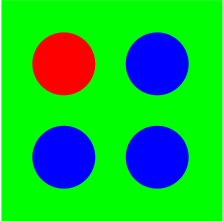
\includegraphics[width=0.4\linewidth]{fig/marker1.png}
	\caption{Marker 1.}
	\label{fig:mar1}
\end{figure}
For this marker we decided to use color segmentation as our approach. The points we extracted were the centers of the three blue circles.\par
We began by converting the image to HSV colour space, splitting its channels and looking at the hue channel as seen in figure \ref{fig:hue1}. We then took the hue value for the blue areas in the original marker as a reference. We used this value to compute a binary image showing only areas with a hue value very close to the desired blue one. The resulting binary image is shown in figure \ref{fig:bin1}. This isolated the the blue circles from the marker very nicely but left some noise from the blue background elements. To ignore this noise, we took advantage of the circles' shape. We found the contours in this binary image and the radius of their minimum enclosing circle. By comparing this radius to the contour's area, we got a value which quantitatively described the roundness of the contour. By selecting the three roundest contours in the binary image, we obtained the three circles in the marker as seen in figure \ref{fig:src1}.\par
We used this marker to test the simulated visual servoing system. In order for the robot to follow the marker's orientation, the three extracted points must be sorted in a consistent manner. To implement this, we first made the assumption that the points form a triangle whose longest side is always the same one. While this is not true for all out-of-plane rotations, it holds for all the projections in the provided sequences. Following this assumption, we used the point opposite the long side as the first element and used the cross product of the two short sides to sort the remaining two points clockwise.\par
This algorithm finds the points with high precision on each image in the provided sequences. It handles in-plane and out-of-plane rotations and scaling but the colors are somewhat sensitive to ambient light changes. A blue ball or similar in the background would also be very troublesome.\par
The color segmentation approach is appropriate for this problem due to the sharp colors on the marker. Our method for circle detection is also quite robust for this problem due to the fact that the circles are well isolated and that we know beforehand how many to look for.

\begin{figure}
	\centering
	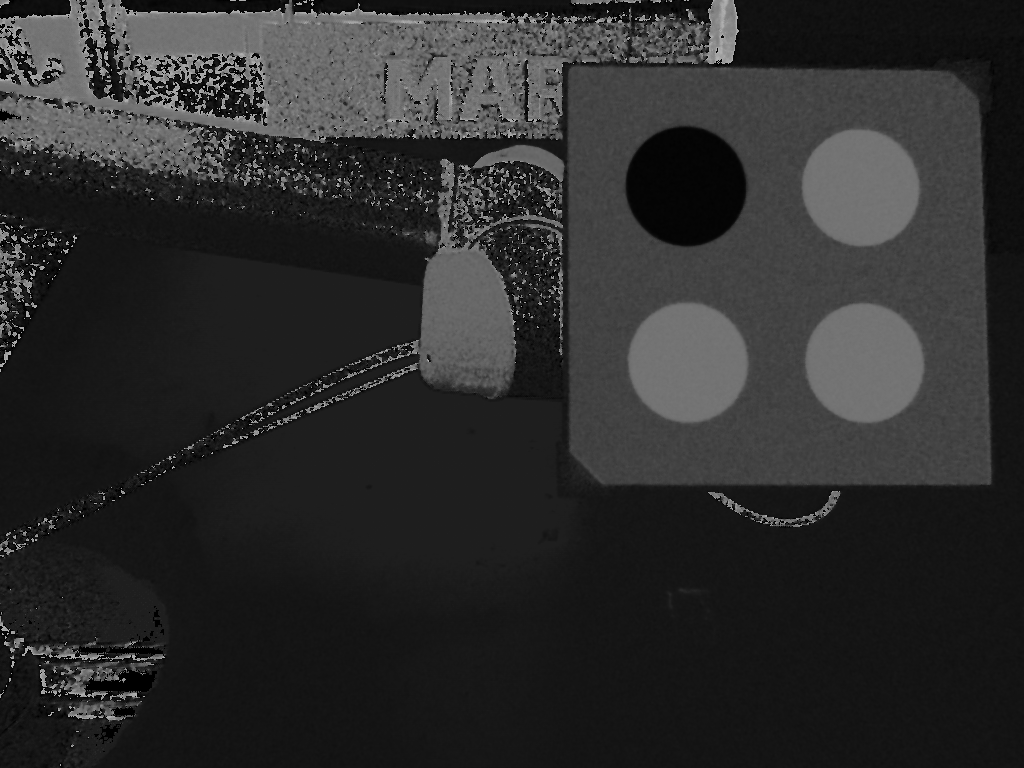
\includegraphics[width=0.7\linewidth]{fig/hue0-1.png}
	\caption{Hue channel of the first image in the color marker sequence.}
	\label{fig:hue1}
\end{figure}

\begin{figure}
	\centering
	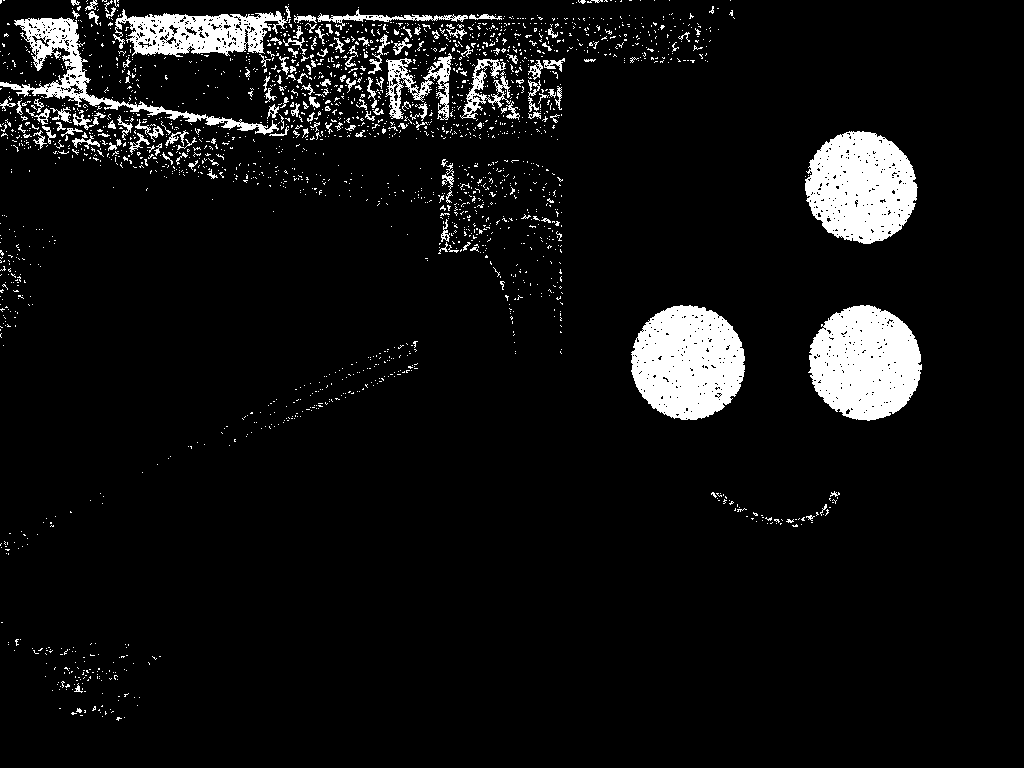
\includegraphics[width=0.7\linewidth]{fig/bin0-1.png}
	\caption{Figure \ref{fig:hue1} after hue thresholding.}
	\label{fig:bin1}
\end{figure}

\begin{figure}
	\centering
	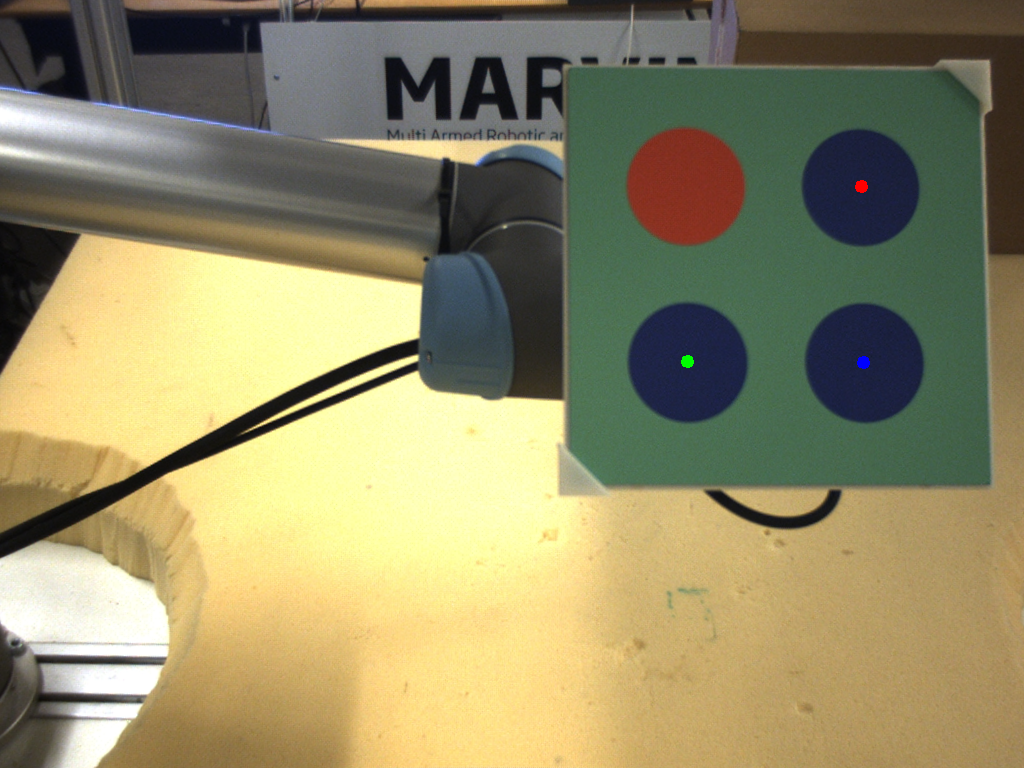
\includegraphics[width=0.7\linewidth]{fig/src0-1.png}
	\caption{Extracted points.}
	\label{fig:src1}
\end{figure}

\newpage
\subsection{Marker 2b}
\begin{figure}
	\centering
	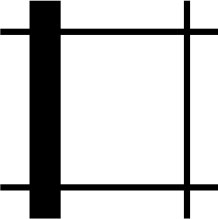
\includegraphics[width=0.4\linewidth]{fig/marker2b.png}
	\caption{Marker 2b.}
	\label{fig:mar2}
\end{figure}
For this marker we used the Hough transformation to find lines in the image. Our target points were the four corners of the white rectangle in the center of the marker.\par
We began by using the Canny algorithm to detect edges in the image as shown in figure \ref{fig:bin2}. We also used the Hough transform to detect the lines as shown in figure \ref{fig:lin2}. We dilated the edges as well as the lines and then combined them using logical AND as seen in figure \ref{fig:and2}. The resulting image shows the marker's lines relatively clearly with some background noise as well. From here we wanted to detect the innermost rectangle in the marker. We made the assumption that this rectangle is the largest one in this binary image. As for the first marker, we found the contours and this time their minimum enclosing rotated rectangle. This is quite a big approximation as it loses precision very quickly for out-of-plane rotations. To make sure we detect a rectangle, we compute a value which quantitatively describes how well the enclosing rectangle fits its corresponding contour. This eliminates most contours apart from the white rectangles in the marker. Finally, we pick the largest remaining rectangle which is our desired one. See figure \ref{fig:src2}.\par
This algorithm finds the desired rectangle for each image in the provided sequences but its precision is subpar for out-of-plane rotations as seen in [REFERENCE FIGURE]. The algorithm handles scaling and in-plane rotation but needs to find a closed contour around the desired rectangle. This makes it sensitive to sharp noise around the edges.\par
The Hough transformation is appropriate for this problem due to the long, sharp edges on the marker. We have chosen parameters for the line detection to maximize our chances to find the lines in the marker. We deal with the large number of false positives by ignoring the lines which don't correspond to edges in the image.\par

\begin{figure}
	\centering
	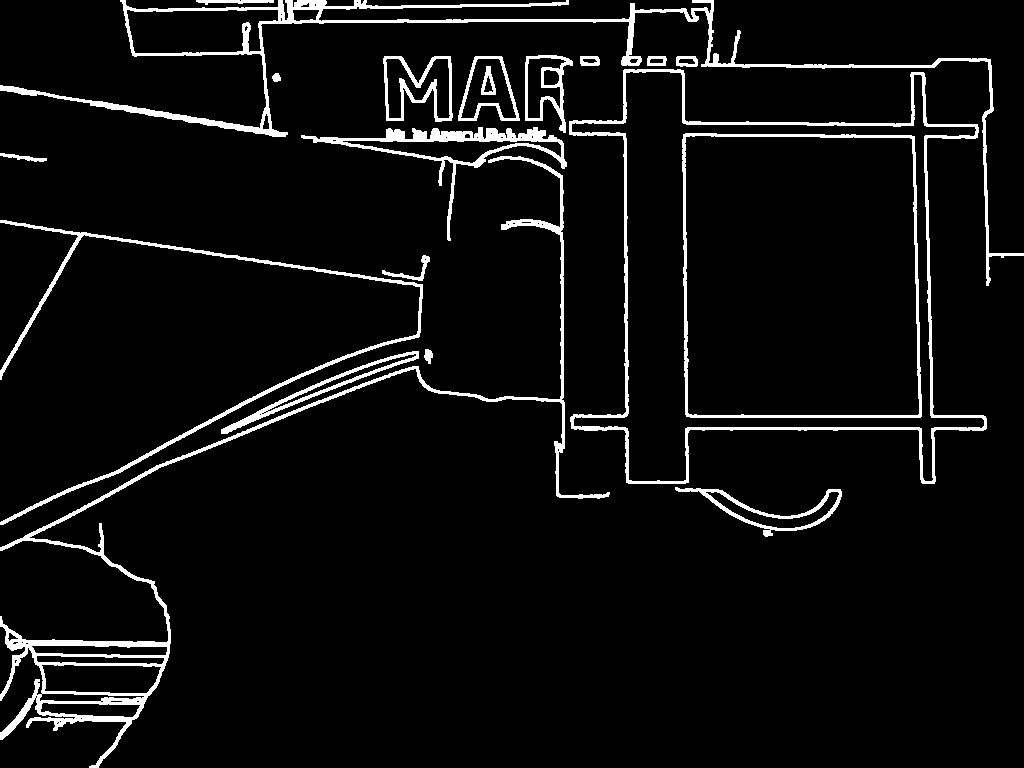
\includegraphics[width=0.7\linewidth]{fig/bin1-1.png}
	\caption{Edges from the first image in the thickline marker sequence.}
	\label{fig:bin2}
\end{figure}

\begin{figure}
	\centering
	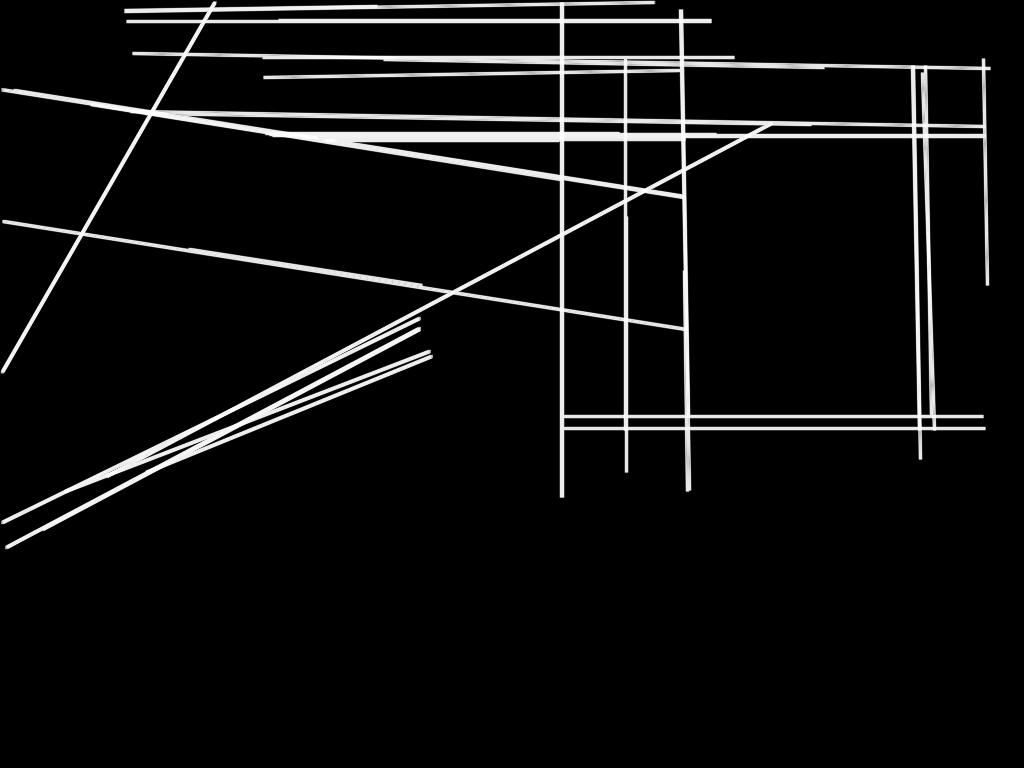
\includegraphics[width=0.7\linewidth]{fig/lin1-1.png}
	\caption{Hough lines from figure \ref{fig:bin2}.}
	\label{fig:lin2}
\end{figure}

\begin{figure}
	\centering
	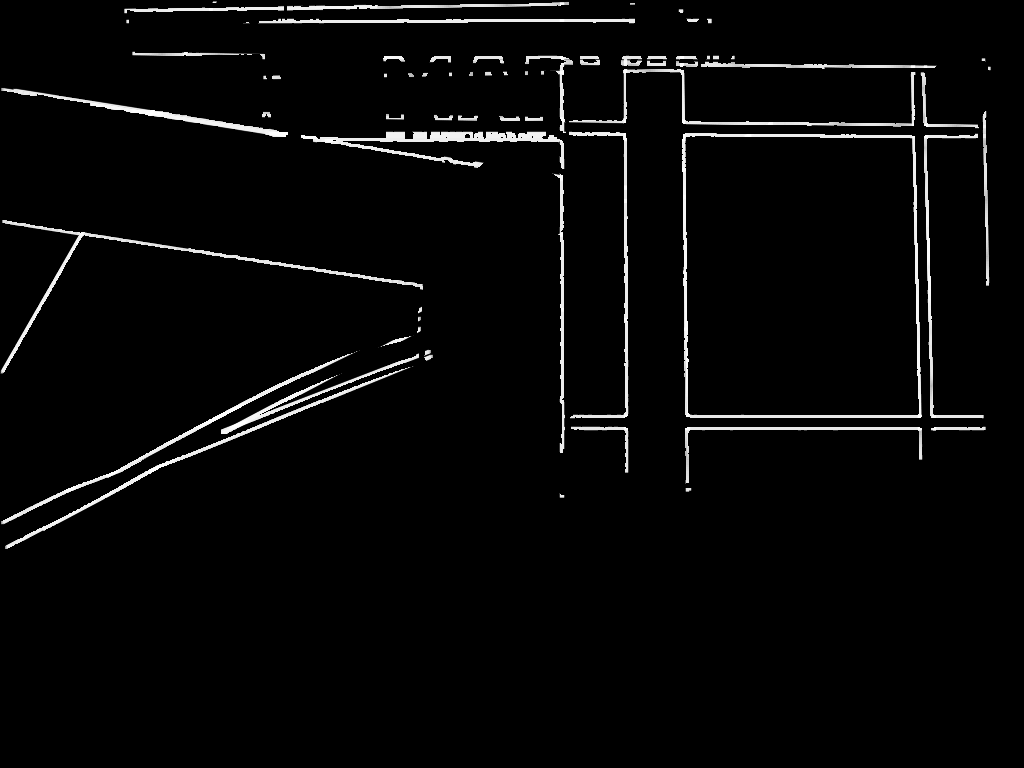
\includegraphics[width=0.7\linewidth]{fig/and1-1.png}
	\caption{Logical AND of figures \ref{fig:bin2} and \ref{fig:lin2}.}
	\label{fig:and2}
\end{figure}

\begin{figure}
	\centering
	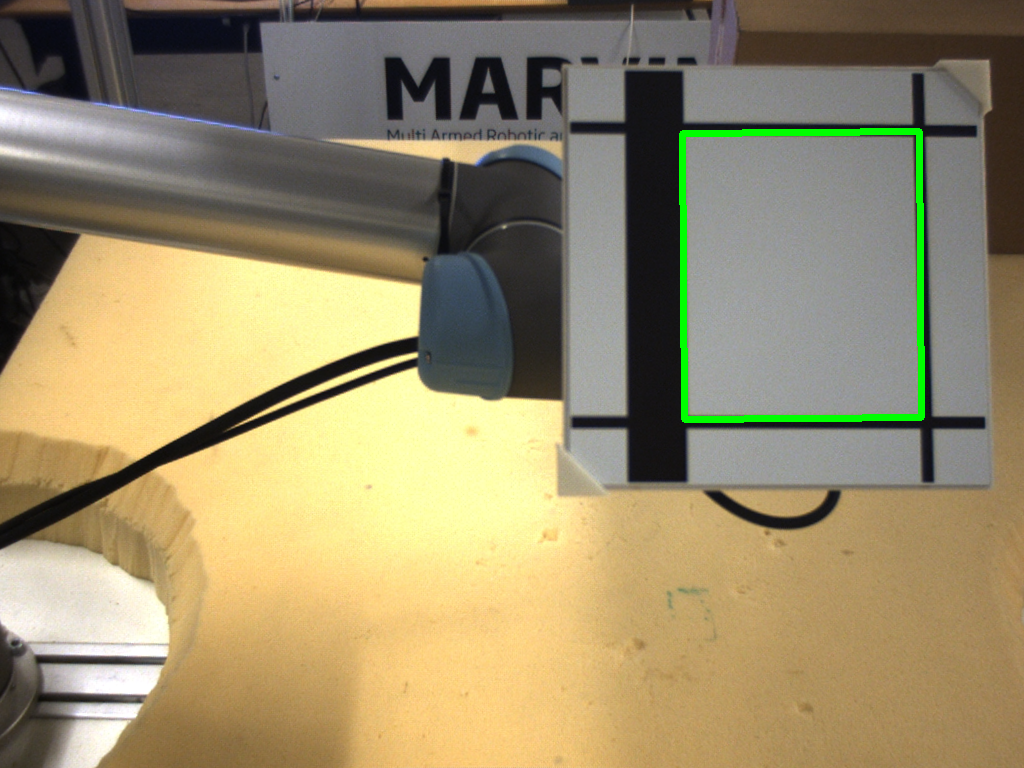
\includegraphics[width=0.7\linewidth]{fig/src1-1.png}
	\caption{Rectangle consisting of the four extracted points.}
	\label{fig:src2}
\end{figure}

\clearpage
\section{Tracking points using image Jacobian}
We have implemented algorithm for visual servoing in this part. For this part we selected specific marker points as described in problem statement and use mathematical camera model to get image pixel coordinates of the points. Image recognition thus wasn't used in this part.

To compute joint updates it was first needed to compose matrix $\boldsymbol{Z}_{image}$ as described in Robotics Notes:
\begin{align}
	\boldsymbol{Z}_{image}(\boldsymbol{q}) = \boldsymbol{J}_{image}\boldsymbol{S}(\boldsymbol{q})\boldsymbol{J}(\boldsymbol{q})\; 
\end{align}
where $\boldsymbol{J}(\boldsymbol{q})$ is manipulator Jacobian. For its computation we used function from RobWork library. $\boldsymbol{J}_{image}$ is image Jacobian matrix. We implemented function for its computation called \texttt{calculateImageJ} which can be found in the file \texttt{inverseKinematics.cpp}. We used fixed value for $z$ coordinate. Since we used frame \texttt{cameraSim} to model the camera we set $z\, = \, -0.5$ for every function call. Finally matrix $\boldsymbol{S}(\boldsymbol{q})$ was composed by inserting transpose of the rotational matrix $\boldsymbol{R}_{base}^{tool}$ twice to its diagonal.

The next information necessary to compute joints updates is difference or move of target points $\overrightarrow{\boldsymbol{dU}}_{image}$. We have programmed function \texttt{calculate\_dUImage} to solve for $\overrightarrow{\boldsymbol{dU}}_{image}$.

Having matrix $\boldsymbol{Z}_{image}$ and $\overrightarrow{\boldsymbol{dU}}_{image}$ it was possible to solve for joint positional update ${\boldsymbol{dq}}$ using method of Linear Least Squares.

We adapted two equations from robotics notes into single expression for ${\boldsymbol{dq}}$ computation:
\begin{align}
	\boldsymbol{dq} = \boldsymbol{Z}^T\left(\boldsymbol{Z}\boldsymbol{Z}^T\right)^{-1} \overrightarrow{\boldsymbol{dU}}_{image}
\end{align}
In this equation we used $\boldsymbol{Z}$ to denote $\boldsymbol{Z}_{image}$.
For this solving of this LSM problem we have implemented function \texttt{compute\_dQ\_LSM} which can be found in \texttt{inverseKinematics.cpp}.

\texttt{algorithm2} is the function, where are all of described functions organized together to compute joint updates $\boldsymbol{dq}$ base on the manipulator state and the error in image coordinates $\overrightarrow{\boldsymbol{dU}}_{image}$.

We have implemented $J_{image}$ and $\overrightarrow{\boldsymbol{dU}}_{image}$ composition in a scalable way, so the same functions can be used to track one or multiple target points.

Model of the robot manipulator has velocity limits on joint movements, so it was necessary to check if the limits were satisfied before joint updates. We did so by measuring time for inverse kinematics computations $\tau_1$, subtracting this time from workcell update period specified by $\Delta T \longleftrightarrow$ \texttt{deltaT} and finally we divided update $\boldsymbol{dq}$ by the result of subtraction. Velocity of joint movement is the result of the operation:
\begin{align}
	\boldsymbol{\dot{q}} = \frac{\boldsymbol{dq}}{dt} = \frac{\boldsymbol{dq}}{\Delta T\, -\, \tau_1}
\end{align}
By comparing the actual velocity with manipulator limits it was possible to find out if the limits are satisfied. If they aren't algorithm simply saturate joint movement in order to hold all conditions. For comparison and saturation, function \texttt{saturateDQ} was implemented.

In the following section we provide simulation results from tests of inverse kinematics.

\subsection{Simulation Tests}
During simulations, we recorded joint configurations, tool/camera frame position and orientation for $\texttt{deltaT} = 1000 ms$ and finally we performed tests for different values for \texttt{deltaT} in the range $50\, ms < \texttt{deltaT} < 1000\, ms$ and plotted maximum errors of 
$\overrightarrow{\boldsymbol{dU}}_{image}$

\subsubsection*{Slow Marker Sequence}
\begin{figure}[!htp]
	% Maximum length
	\subfloat[Tracking Single Point]
	{
		\label{fig:Slow1PointJoints}
		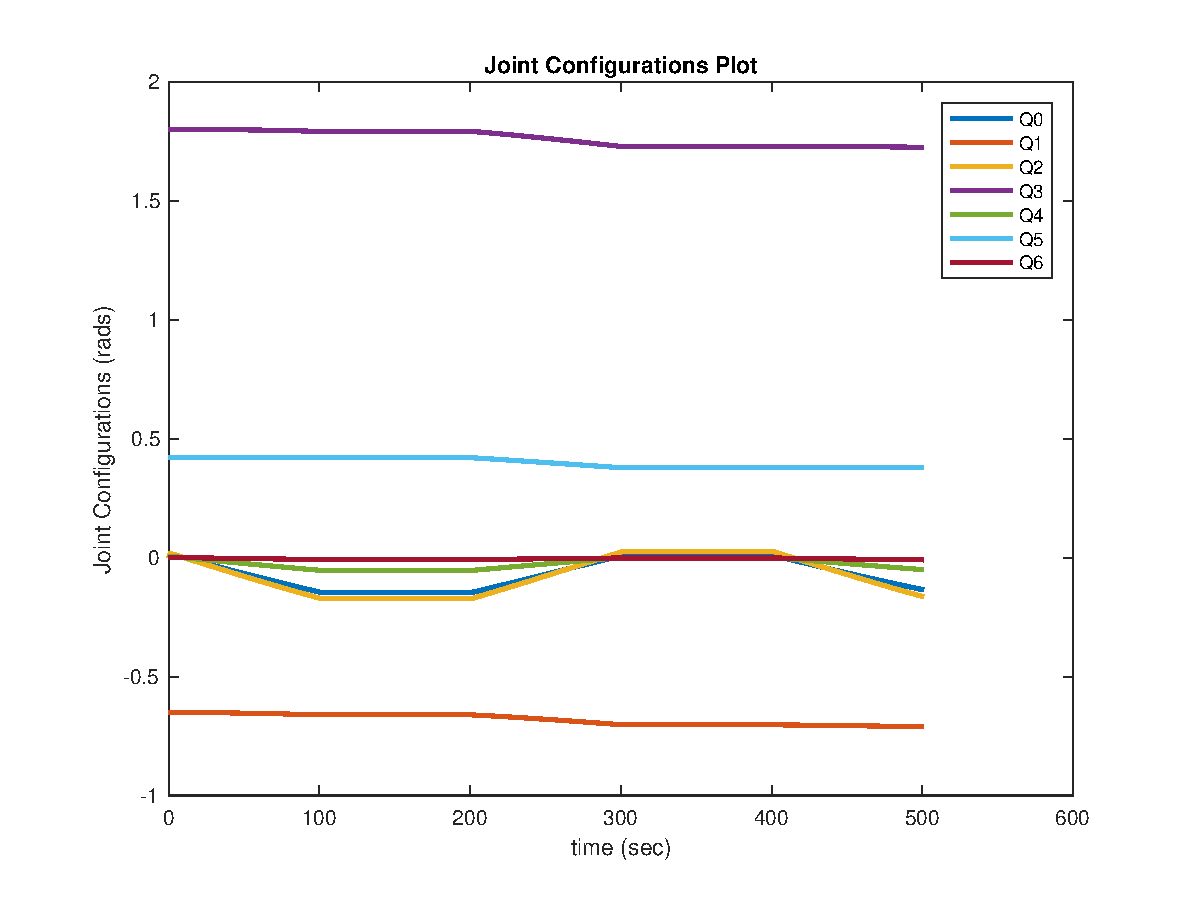
\includegraphics[width=0.49\linewidth]{fig/SlowSequence_joints_1_Targ_Pt.eps}
	}\hfill
	\subfloat[Tracking 3 Points]
	{
		\label{fig:Slow3PointsJoints}
		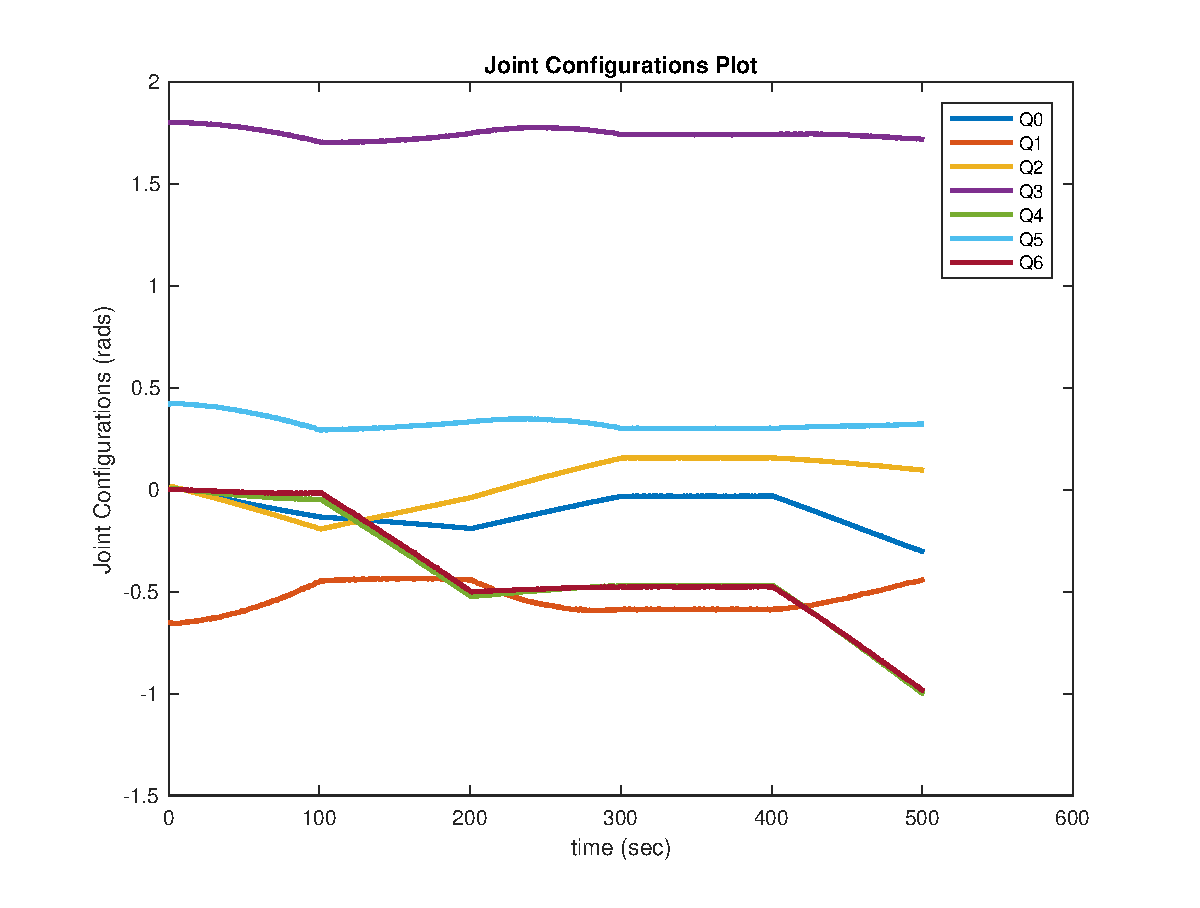
\includegraphics[width=0.49\linewidth]{fig/SlowSequence_joints_M_Targ_Pts.eps}
	}%
	\caption{Joint configurations}
	\label{fig:SlowSequenceJoints}
\end{figure}
There are differences between joint coordinates for tracking single and 3 target points in the graphs \ref{fig:Slow1PointJoints} and \ref{fig:Slow3PointsJoints}. The reason behind this is following. When the manipulator is tracking single point, it just follow its position. There is no orientation information about the marker when using single tracking point. Whereas during following of 3 target points, orientation of the marker gains important role, as the manipulator is trying to rotate its tool/camera frame to align its position and orientation with the marker. 

\begin{figure}[!h]
	% Maximum length
	\subfloat[Tracking Single Point]
	{
		\label{fig:Slow1PointToolPose}
		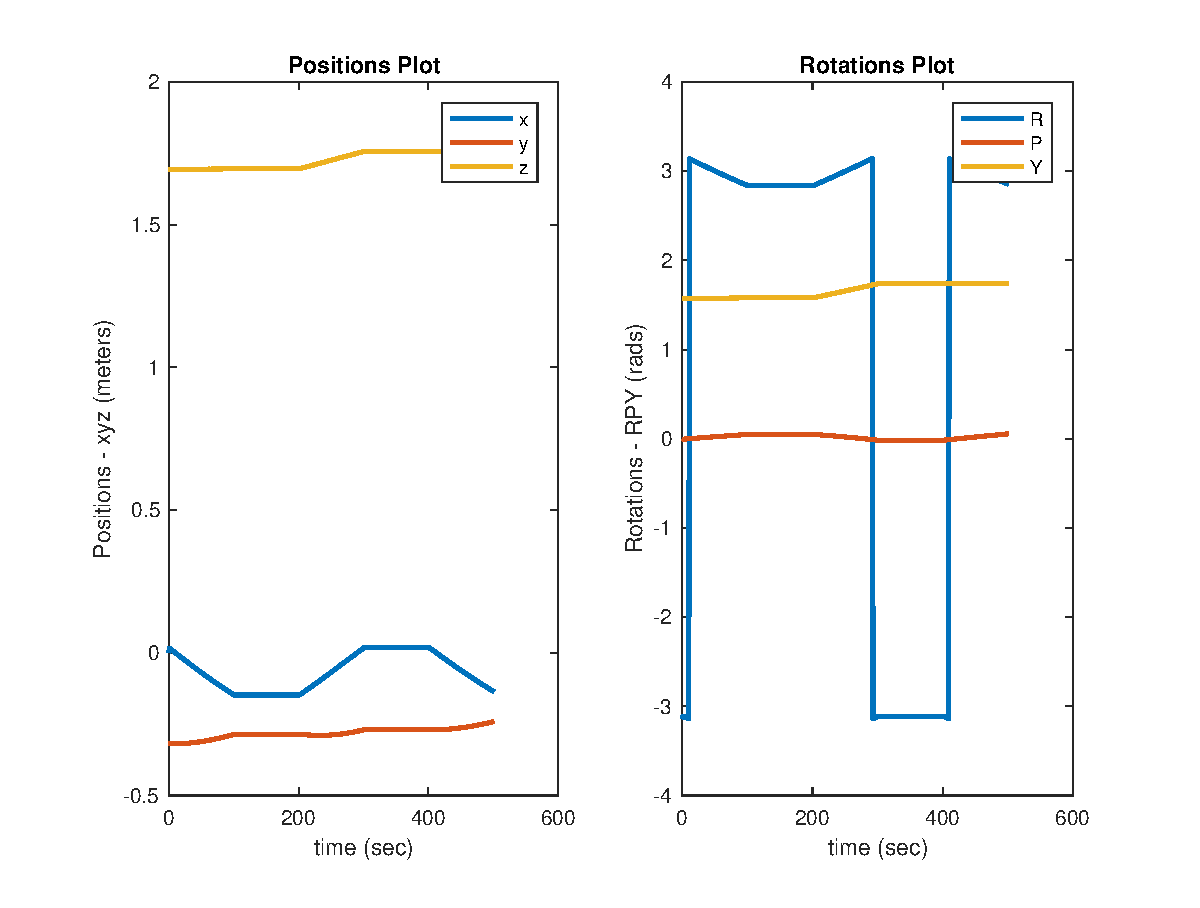
\includegraphics[width=0.49\linewidth]{fig/SlowSequence_tool_pose_1_Targ_Pt.eps}
	}\hfill
	\subfloat[Tracking 3 Points]
	{
		\label{fig:Slow3PointsToolPose}
		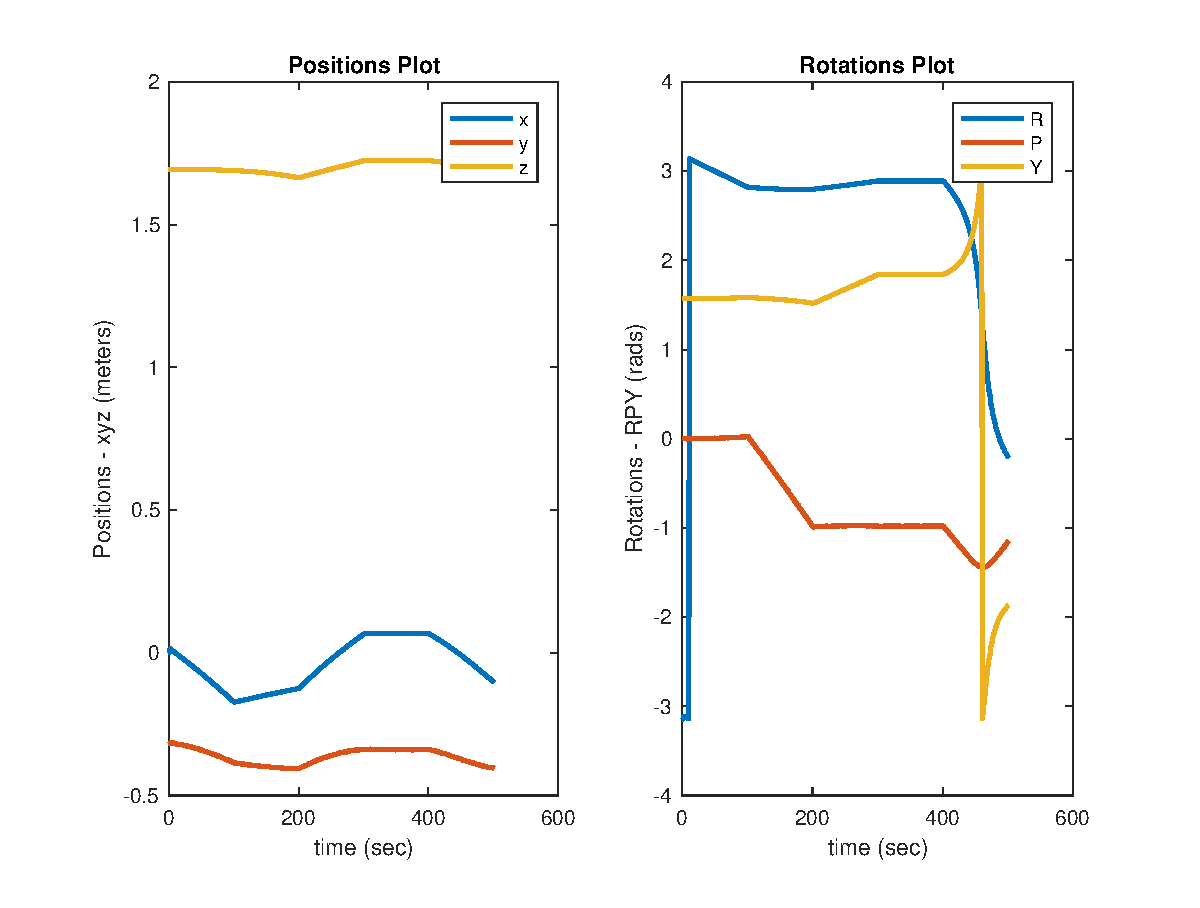
\includegraphics[width=0.49\linewidth]{fig/SlowSequence_tool_pose_M_Targ_Pts.eps}
	}%
	\caption{Tool pose transformations}
	\label{fig:SlowSequenceToolPose}
\end{figure}
In figure \ref{fig:Slow1PointToolPose} and \ref{fig:Slow3PointsToolPose} are apparent jumps in roll angle around $z$ axis. This however doesn't imply jumps in tool orientation. Abrupt jumps in the graphs were caused because of switching between $-\pi$ and $\pi$ rad angle. In the real world, change in orientation is small. Implementation of Robwork transformations probably keeps all orientation angles in the interval $ \langle -\pi, \; \pi \rangle $.

\vspace{0.5cm}
\textbf{Simulation for different $\Delta T$s} \\
\begin{figure}
	\centering
	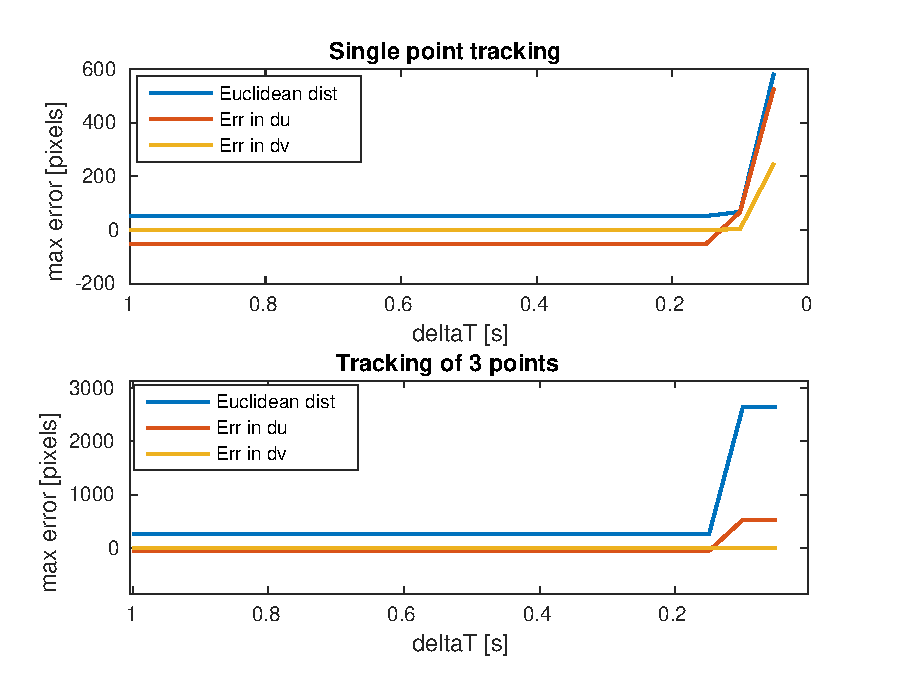
\includegraphics[width=0.7\linewidth]{fig/SlowSequence_errors.eps}
	\caption{Maximum errors during Slow Sequence Marker following}
	\label{fig:SlowSequence_errors}
\end{figure}

\vspace{0.5cm}
\textbf{Simulation for different $\Delta T$s} \\
\begin{figure}
	\centering
	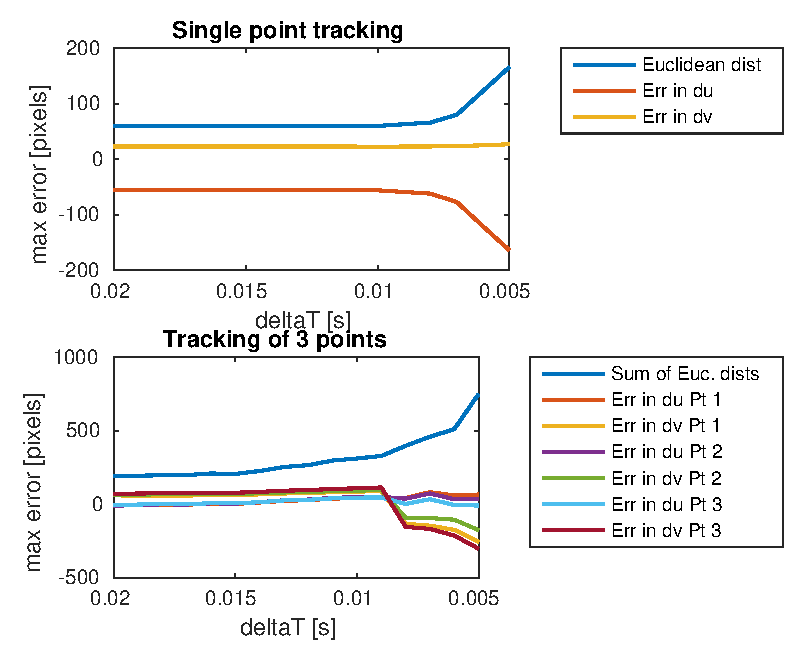
\includegraphics[width=0.7\linewidth]{fig/SlowSequence_low_dTs_errors.eps}
	\caption{Maximum errors during Slow Sequence Marker following}
	\label{fig:SlowSequence_low_dTs_errors}
\end{figure}

There are plotted maximum pixel errors on the figure \ref{fig:SlowSequence_errors}.

For timing purposes we used C++ Chrono library, for taking time instant of start of the computation of updates and the end instant. For differentiation of joint updates and subsequently getting of velocity, we used difference of these two time stamps divided time which left for joints update. 

As you can see on the figure \ref{fig:SlowSequence_errors} we didn't reach manipulator velocity limits in the interval $\Delta T \, \in \langle0.05, 1\rangle \, [s]$ as was described in the problem statement.

For this reason we lowered the interval to the $\Delta T \, \in \langle0.005, 0.02\rangle \, [s]$. And in this case, there is apparent increase in the maximum errors for low $\Delta T$. Results are plotted in the figure \ref{fig:SlowSequence_low_dTs_errors}.

Due to non-real time OS, results might be different for each simulation and doesn't offer precise information. However for the purpose of the school exercise, we were able to limit joints speed velocities according to problem statement.


\subsubsection*{Medium Marker Sequence}
The same problems and explanation apply for the Medium marker sequence. Joint coordinates and tool positions are plotted on the graphs \ref{fig:MediumSequenceJoints} and \ref{fig:MediumSequenceToolPose}. Only difference from Slow sequence is in the time axis. Due to faster and larger movements time span is shorter.
\begin{figure}[!htp]
	% Maximum length
	\subfloat[Tracking Single Point]
	{
		\label{fig:Medium1PointJoints}
		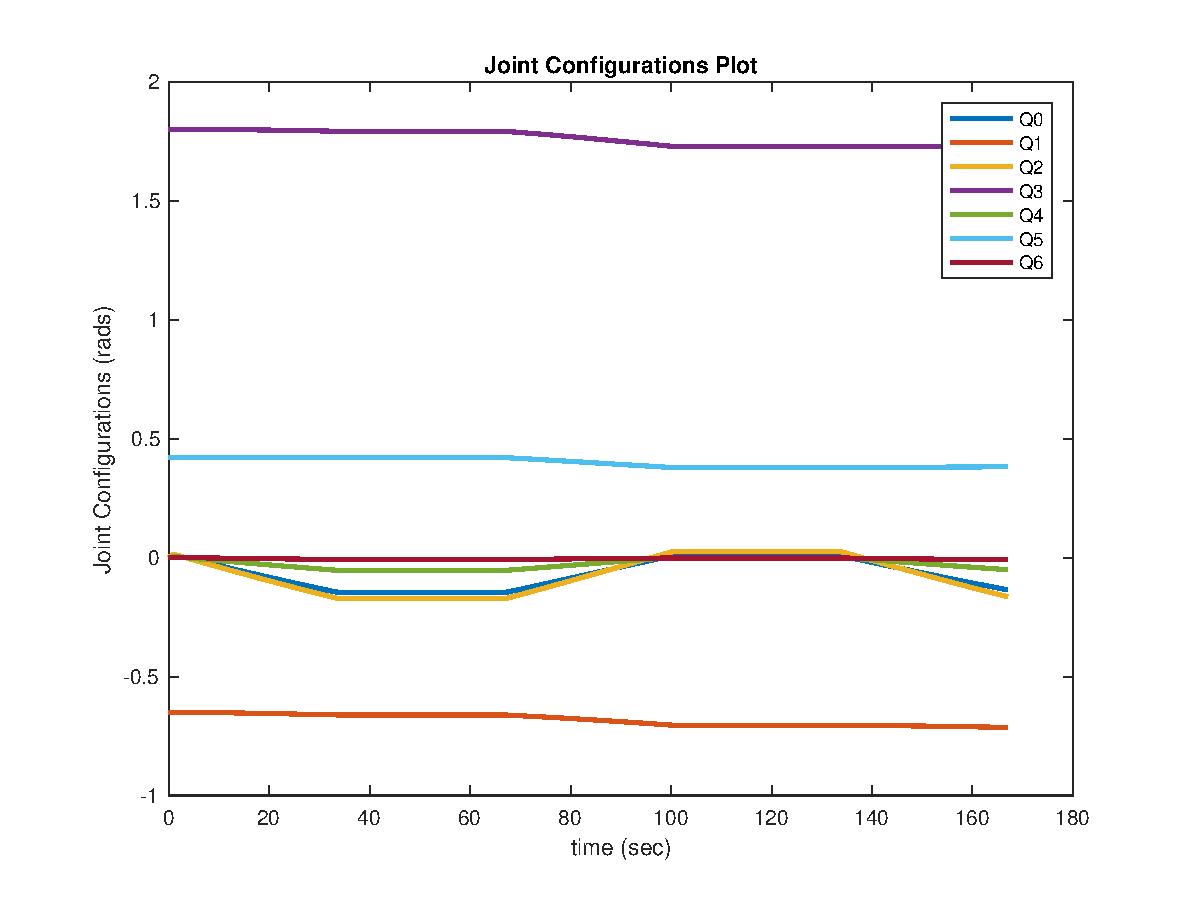
\includegraphics[width=0.49\linewidth]{fig/MediumSequence_joints_1_Targ_Pt.eps}
	}\hfill
	\subfloat[Tracking 3 Points]
	{
		\label{fig:Medium3PointsJoints}
		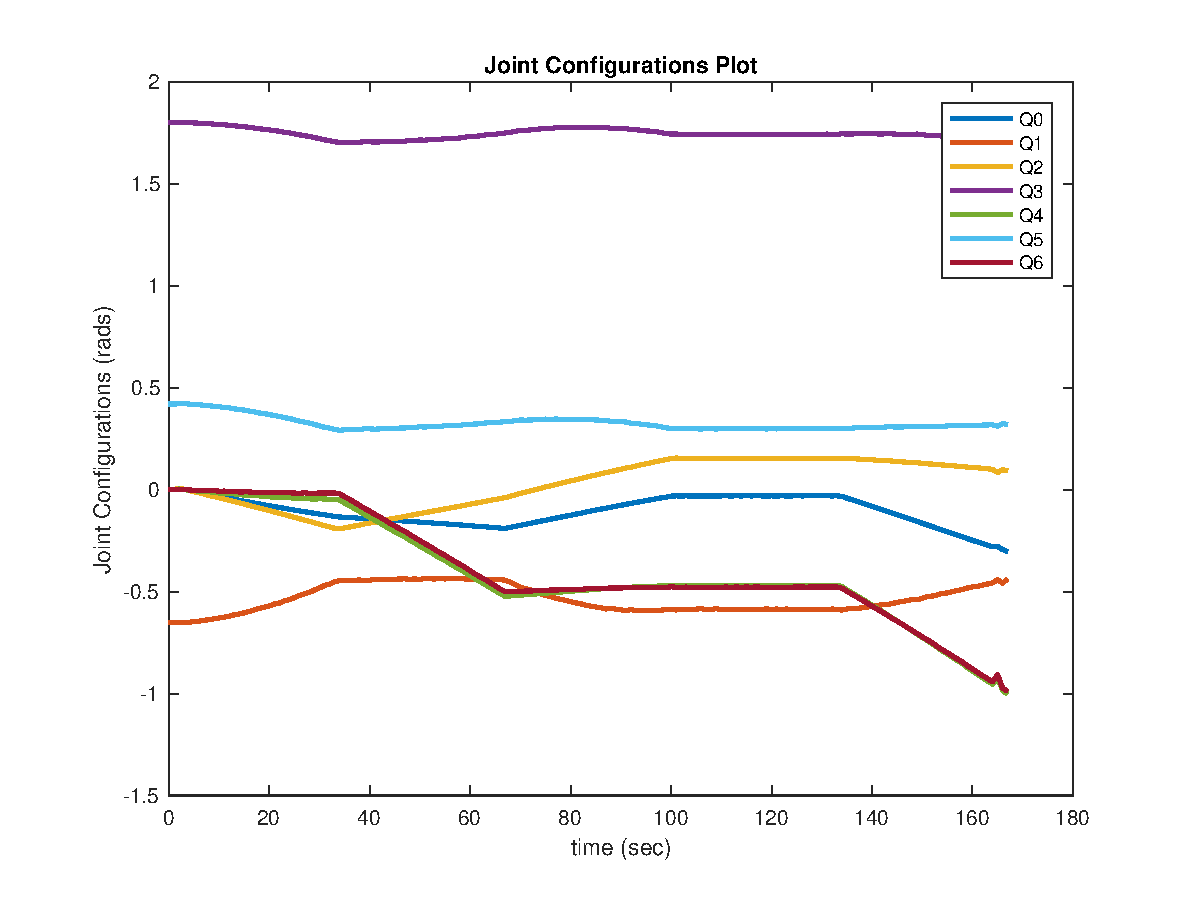
\includegraphics[width=0.49\linewidth]{fig/MediumSequence_joints_M_Targ_Pts.eps}
	}%
	\caption{Joint configurations}
	\label{fig:MediumSequenceJoints}
\end{figure}

\begin{figure}[!htp]
	% Maximum length
	\subfloat[Tracking Single Point]
	{
		\label{fig:Medium1PointToolPose}
		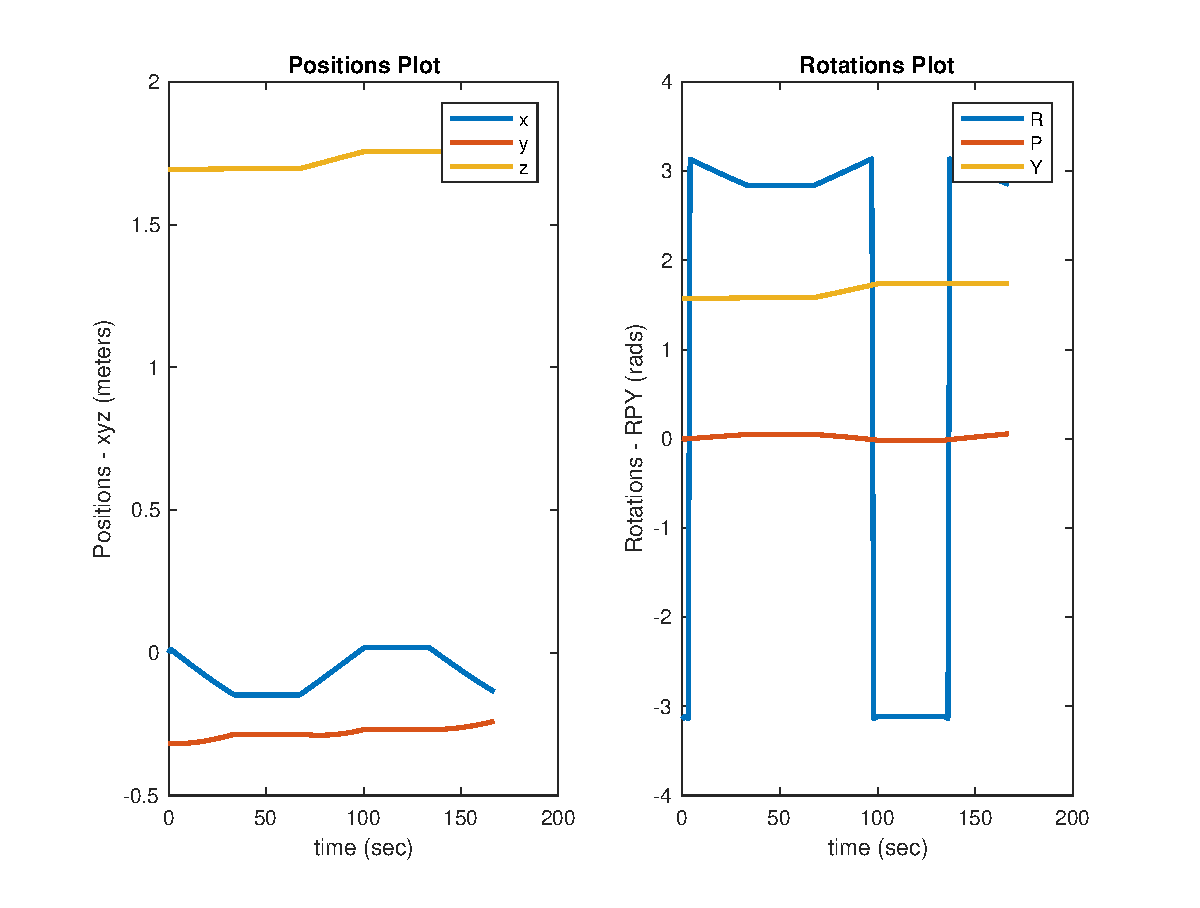
\includegraphics[width=0.49\linewidth]{fig/MediumSequence_tool_pose_1_Targ_Pt.eps}
	}\hfill
	\subfloat[Tracking 3 Points]
	{
		\label{fig:MediumPointsToolPose}
		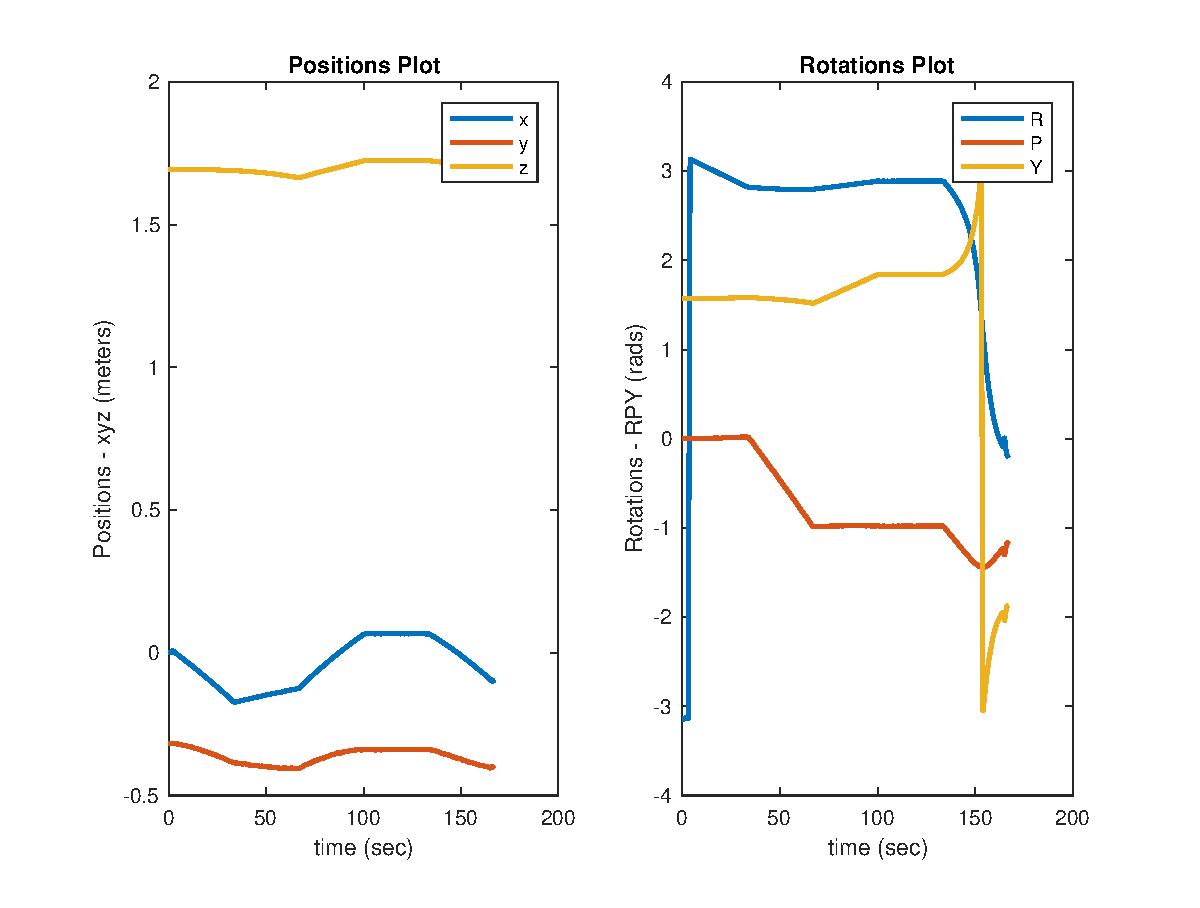
\includegraphics[width=0.49\linewidth]{fig/MediumSequence_tool_pose_M_Targ_Pts.eps}
	}%
	\caption{Tool pose transformations}
	\label{fig:MediumSequenceToolPose}
\end{figure}

\vspace{0.5cm}
\textbf{Simulation for different $\Delta T$s} \\
\begin{figure}
	\centering
	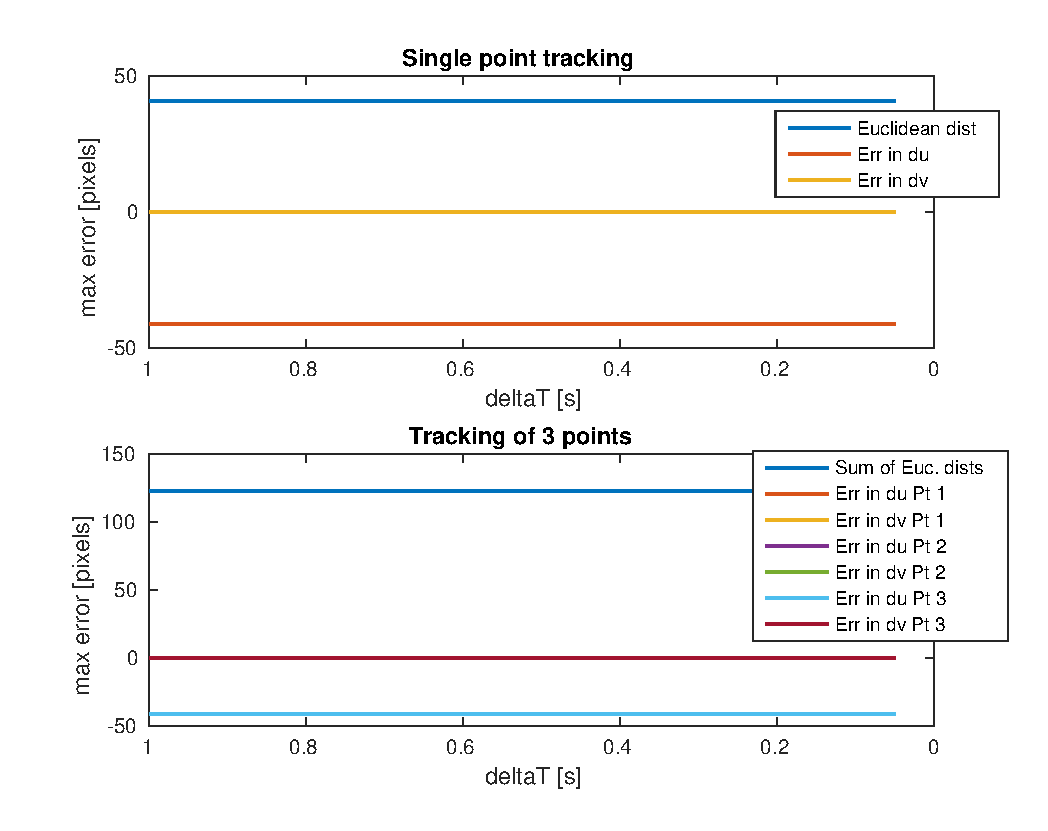
\includegraphics[width=0.7\linewidth]{fig/MediumSequence_errors.eps}
	\caption{Maximum errors during Medium Sequence Marker following}
	\label{fig:MediumSequence_errors}
\end{figure}
\begin{figure}
	\centering
	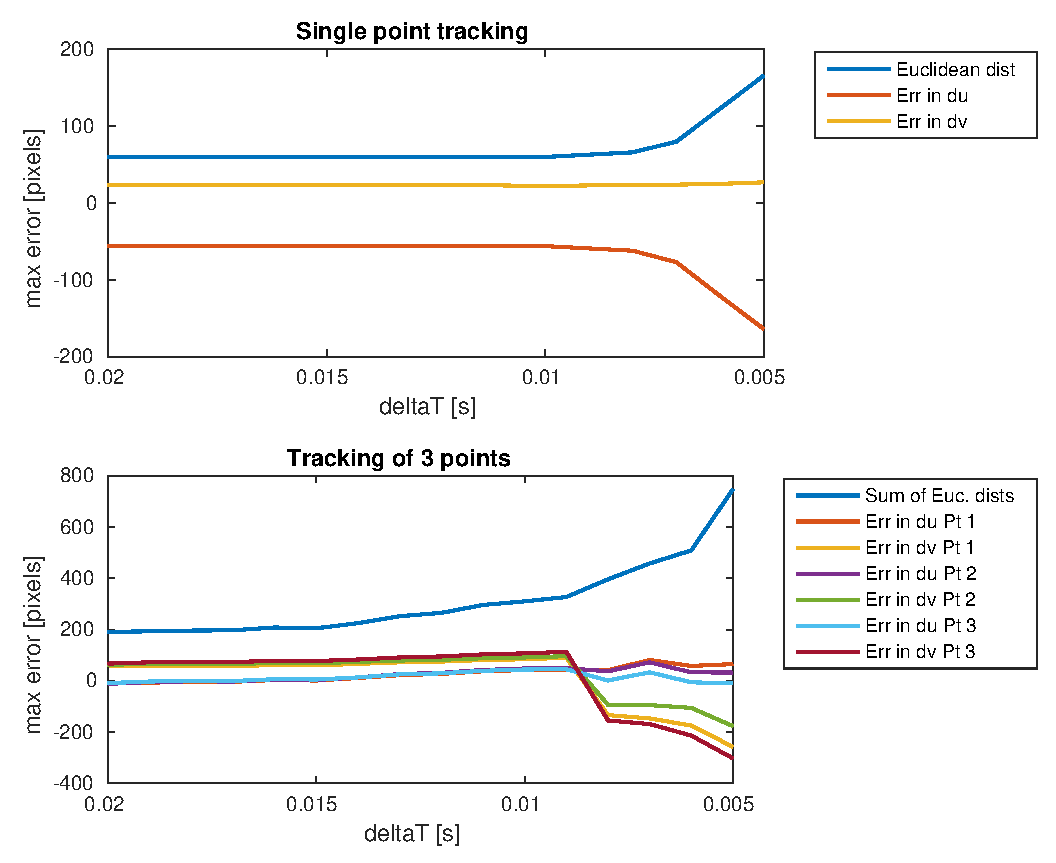
\includegraphics[width=0.7\linewidth]{fig/MediumSequence_low_dTs_errors.eps}
	\caption{Maximum errors during Medium Sequence Marker following}
	\label{fig:MediumSequence_low_dTs_errors}
\end{figure}
There are plotted maximum pixel errors on the figure \ref{fig:MediumSequence_errors}. Again, we didn't reach manipulator velocity limits in the original interval. Results after lowering the interval of $\Delta T$ are plotted in the figure \ref{fig:MediumSequence_low_dTs_errors}.

We have to state the same as for the preceding test. All timing tests were performed on the regular laptop PC, running non-real time operating system. So results from another tests can differ.

\subsubsection*{Fast Marker Sequence}
Joint coordinates and tool positions are plotted on the graphs \ref{fig:FastSequenceJoints} and \ref{fig:FastSequenceToolPose}. Span of time axis is again shorter.

\begin{figure}[!htp]
	% Maximum length
	\subfloat[Tracking Single Point]
	{
		\label{fig:Fast1PointJoints}
		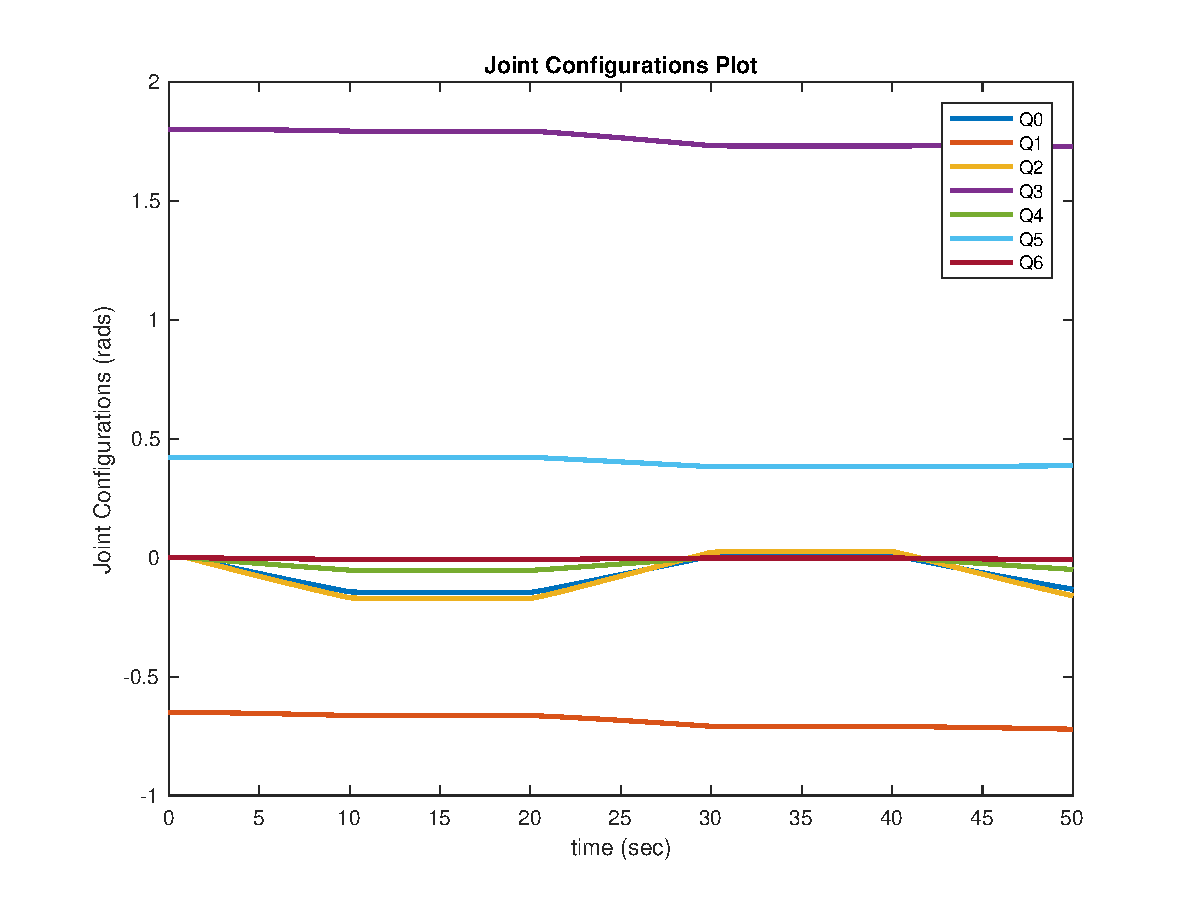
\includegraphics[width=0.49\linewidth]{fig/FastSequence_joints_1_Targ_Pt.eps}
	}\hfill
	\subfloat[Tracking 3 Points]
	{
		\label{fig:Fast3PointsJoints}
		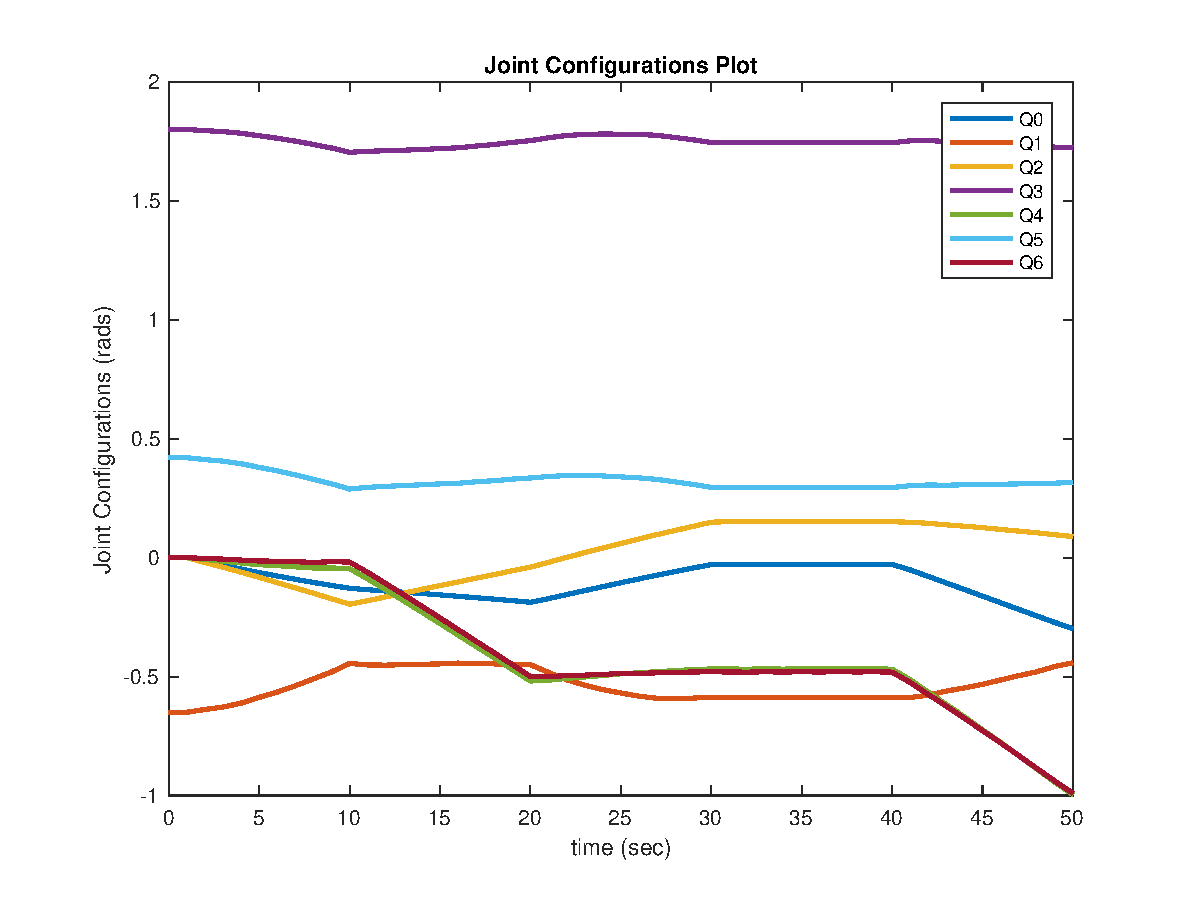
\includegraphics[width=0.49\linewidth]{fig/FastSequence_joints_M_Targ_Pts.eps}
	}%
	\caption{Joint configurations}
	\label{fig:FastSequenceJoints}
\end{figure}

\begin{figure}[!htp]
	% Maximum length
	\subfloat[Tracking Single Point]
	{
		\label{fig:Fast1PointToolPose}
		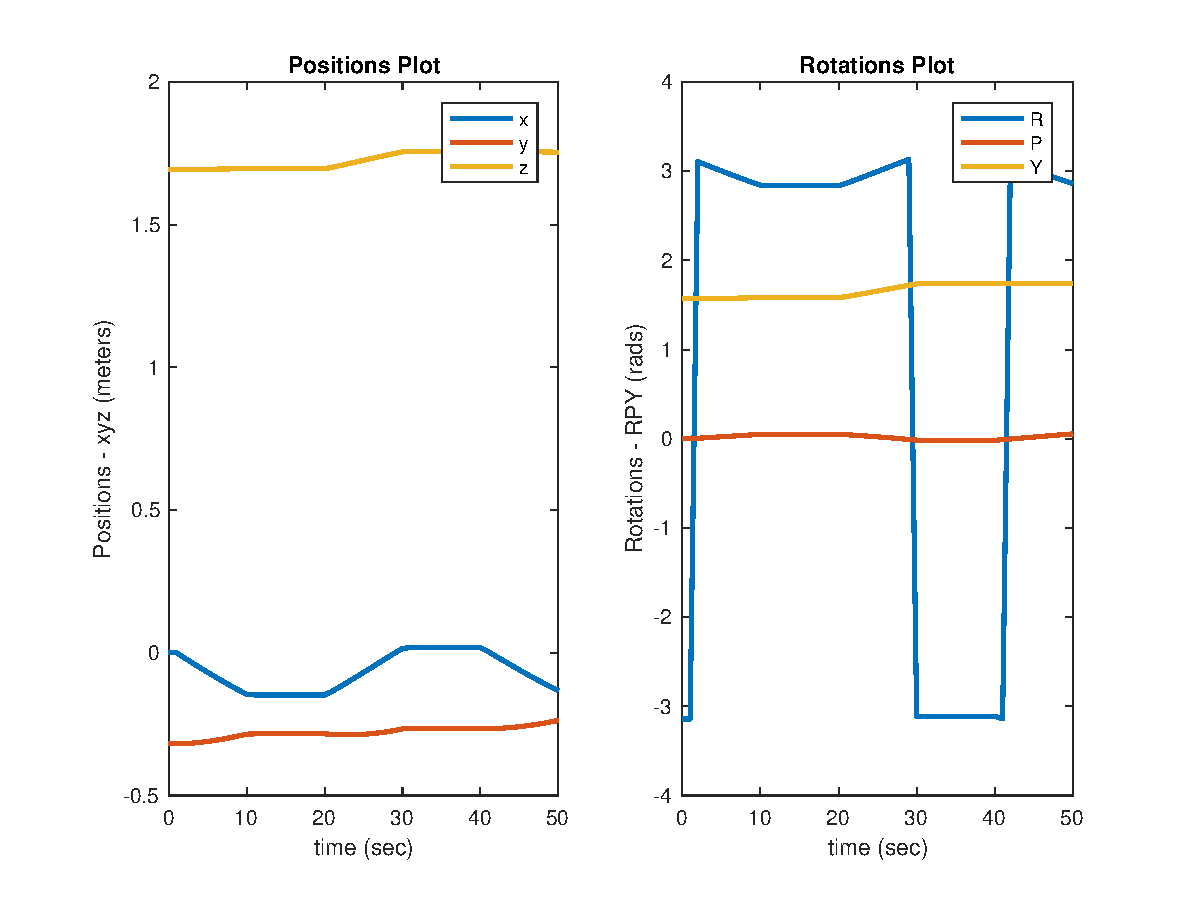
\includegraphics[width=0.49\linewidth]{fig/FastSequence_tool_pose_1_Targ_Pt.eps}
	}\hfill
	\subfloat[Tracking 3 Points]
	{
		\label{fig:FastPointsToolPose}
		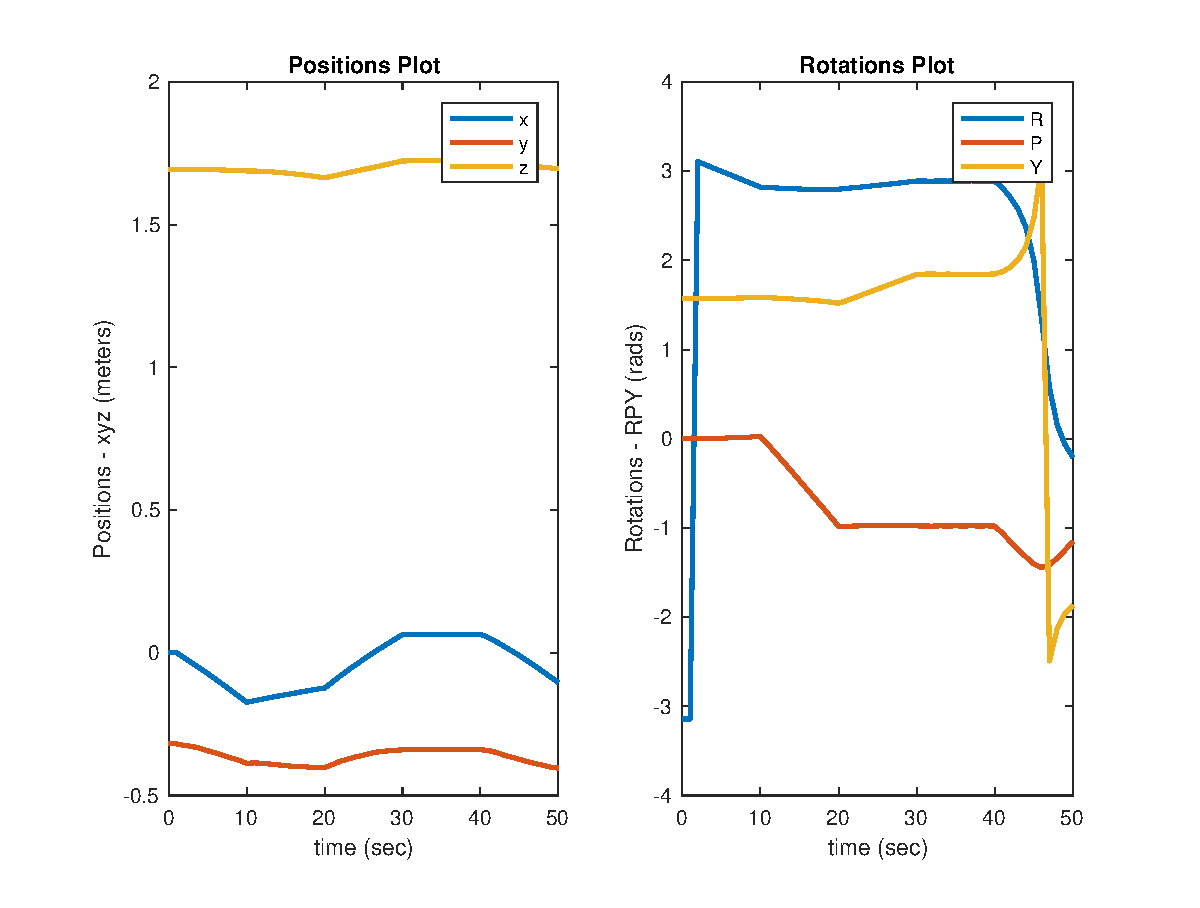
\includegraphics[width=0.49\linewidth]{fig/FastSequence_tool_pose_M_Targ_Pts.eps}
	}%
	\caption{Tool pose transformations}
	\label{fig:FastSequenceToolPose}
\end{figure}

\vspace{0.5cm}
\textbf{Simulation for different $\Delta T$s} \\
\begin{figure}
	\centering
	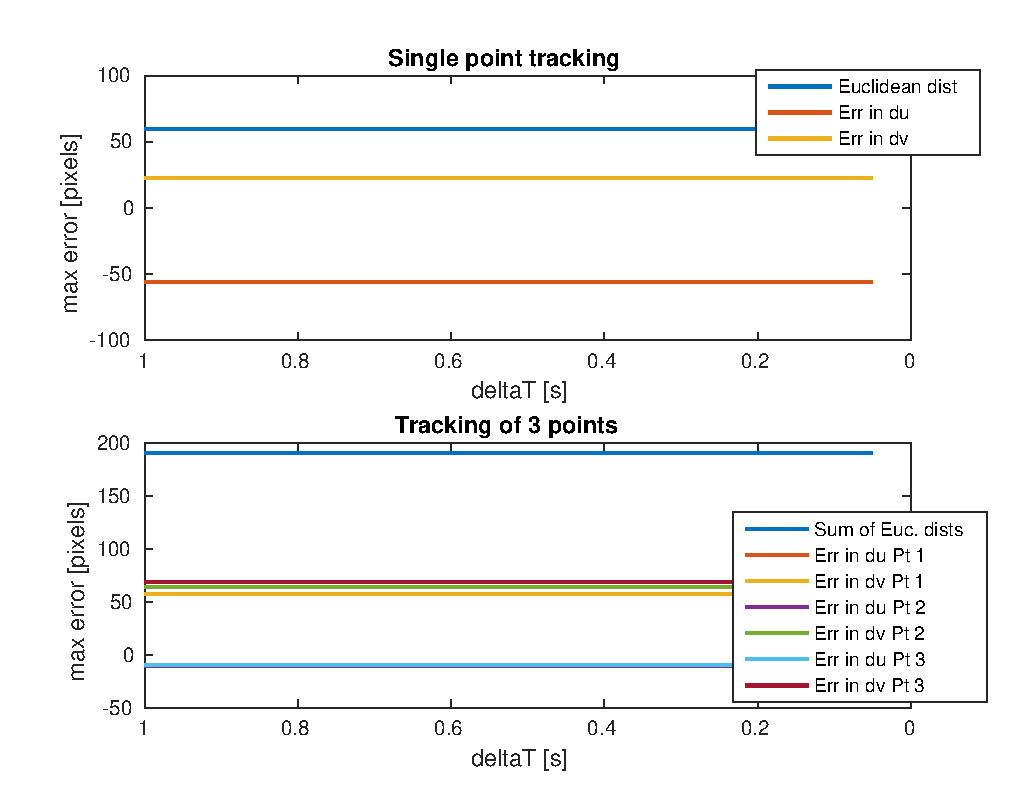
\includegraphics[width=0.7\linewidth]{fig/FastSequence_errors.eps}
	\caption{Maximum errors during Fast Sequence Marker following}
	\label{fig:FastSequence_errors}
\end{figure}

\begin{figure}
	\centering
	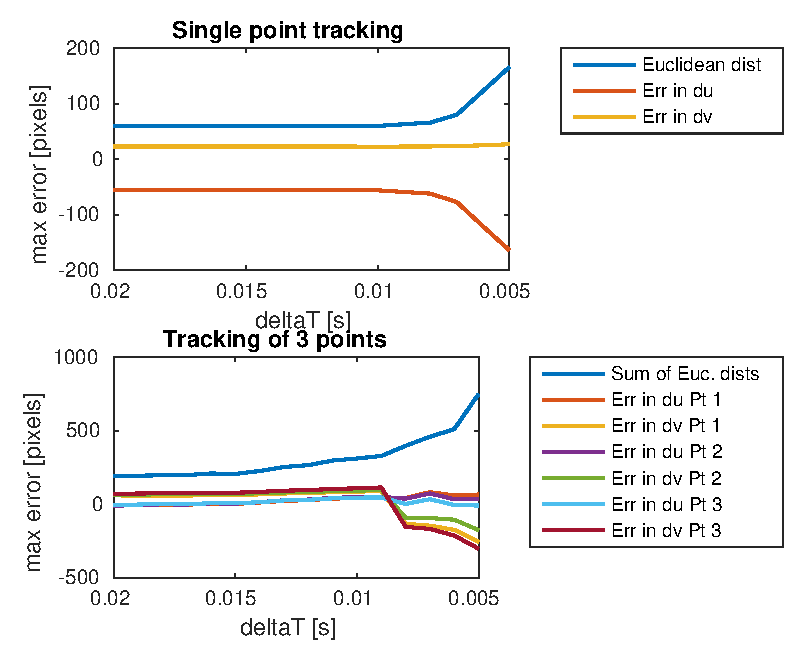
\includegraphics[width=0.7\linewidth]{fig/FastSequence_low_dTs_errors.eps}
	\caption{Maximum errors during Fast Sequence Marker following}
	\label{fig:FastSequence_low_dTs_errors}
\end{figure}

There are plotted maximum pixel errors on the figure \ref{fig:FastSequence_errors} for original interval. Results from simulations for lower interval are plotted on the figure \ref{fig:FastSequence_low_dTs_errors}.

\subsubsection*{Conclusion for different speed sequences}
Even though timing and velocity computation during test simulations wasn't precise due to non-realtime of the OS, we can conclude some final facts. 
Manipulator was able to follow the marker for each sequence with \texttt{deltaT} $ >\, 0.01 s$. The reason behind these results is probably very short time needed for inverse kinematics computations. We found out is in the order of microseconds, whereas simulation were performed for $\Delta T$s which were one order in magnitude larger (miliseconds). These results will be also different when simulated on different computer.

\section{Combining feature extraction and tracking} 
For the last part of the project we have chosen the Marker 1 for image recognition. Image recognition was integrated into Robwork project. All the image recognition function are in the file \texttt{marker1.cpp}. For proper tracking of multiple points, it was necessary to sort the detected points in consistent order for every detection.

After performing of several tests we have found, that recognition time varies among different machines. Average time for one of our computer was around 30 ms whereas on the second one it was just around 25 ms.

For further plots we have chosen one \texttt{deltaT} which don't cause any problems during following. And the second one, which is too short and unsaturated joints velocities are larger than limits.

\begin{figure}[!htp]
	% Maximum length
	\subfloat[Tracking Single Point]
	{
		\label{fig:SlowSequence_dT50_1Pt_following_error_vs_time}
		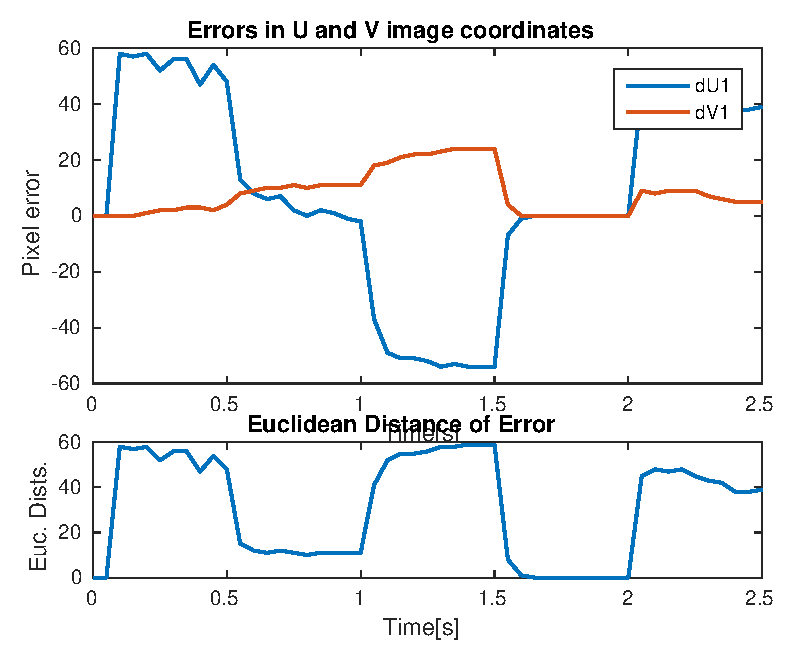
\includegraphics[width=0.49\linewidth]{fig/SlowSequence_dT50_1Pt_following_error_vs_time.eps}
	}\hfill
	\subfloat[Tracking 3 Points]
	{
		\label{fig:SlowSequence_dT50_MPt_following_error_vs_time}
		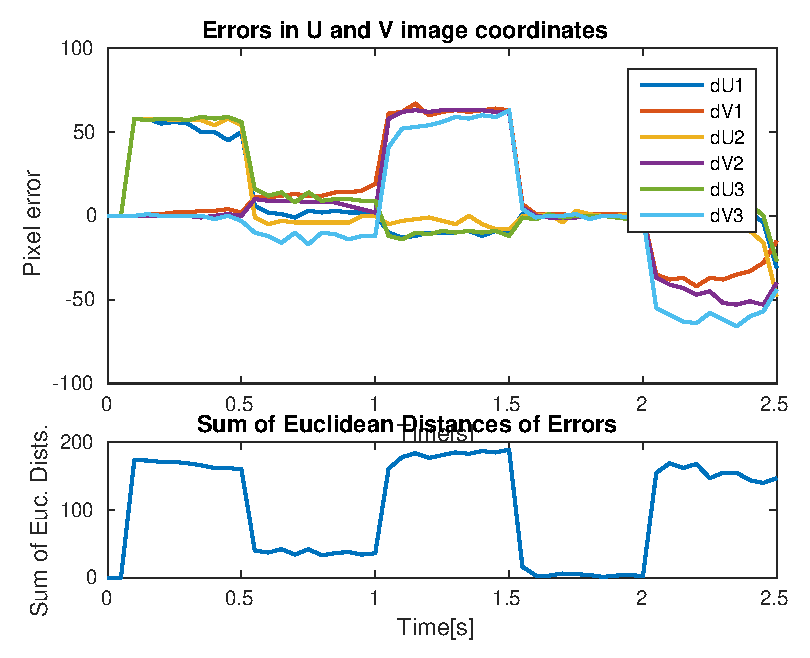
\includegraphics[width=0.49\linewidth]{fig/SlowSequence_dT50_MPt_following_error_vs_time.eps}
	}%
	\caption{Slow Sequence, \texttt{deltaT = 50} ms}
	\label{fig:SlowSequence_dT50_following_error_vs_time}
\end{figure}
\begin{figure}[!htp]
	% Maximum length
	\subfloat[Tracking Single Point]
	{
		\label{fig:SlowSequence_dT35_1Pt_following_error_vs_time}
		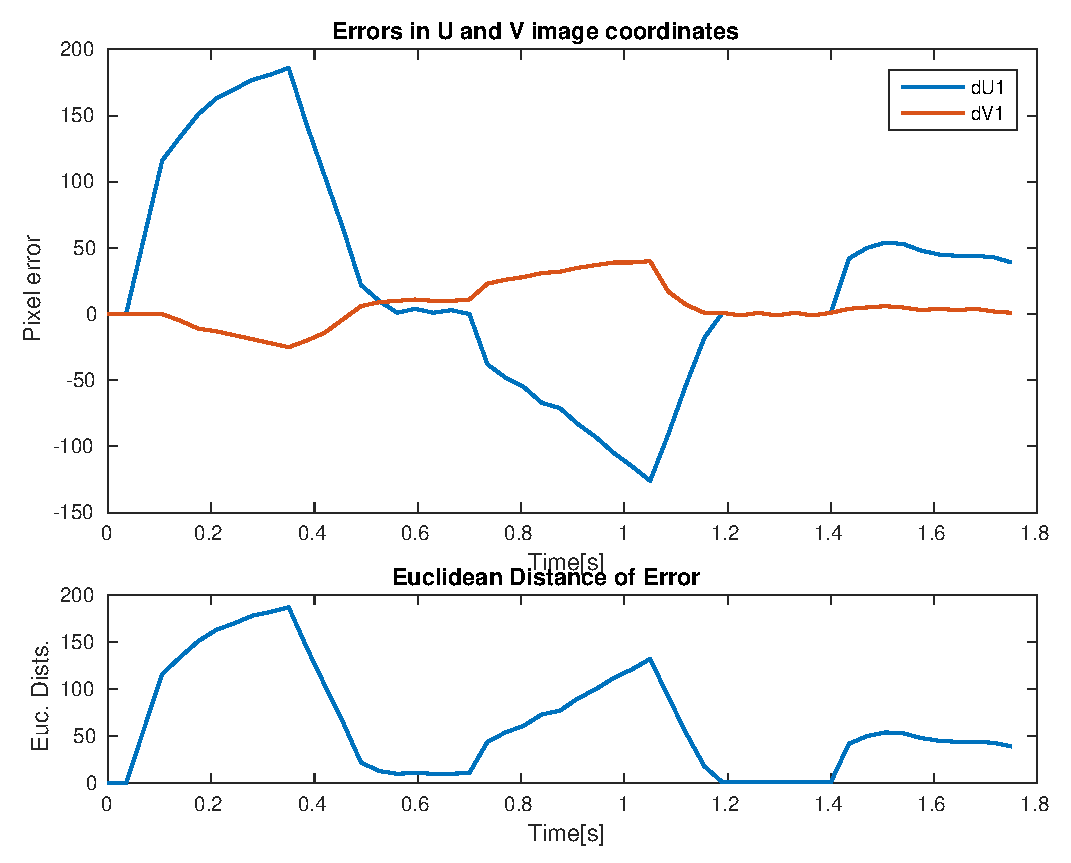
\includegraphics[width=0.49\linewidth]{fig/SlowSequence_dT35_1Pt_following_error_vs_time.eps}
	}\hfill
	\subfloat[Tracking 3 Points]
	{
		\label{fig:SlowSequence_dT35_MPt_following_error_vs_time}
		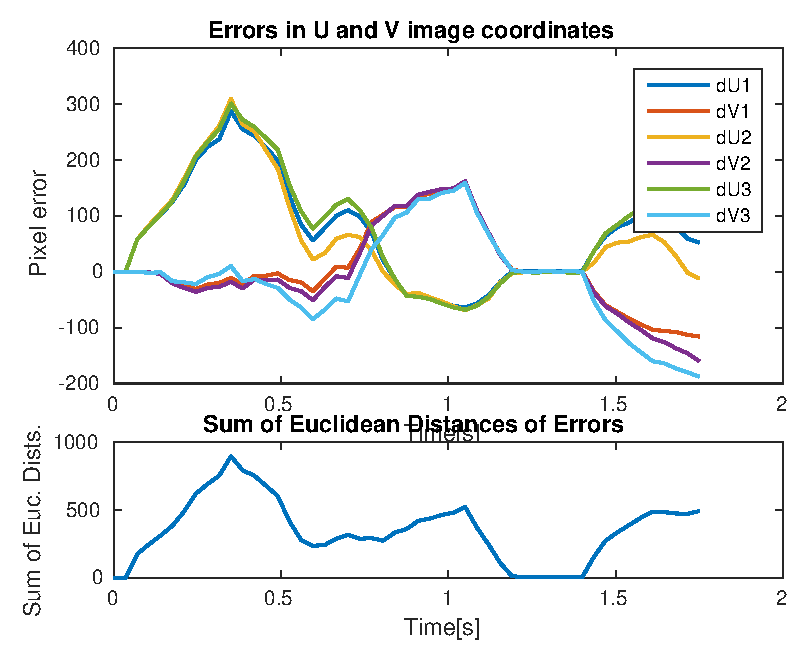
\includegraphics[width=0.49\linewidth]{fig/SlowSequence_dT35_MPt_following_error_vs_time.eps}
	}%
	\caption{Slow Sequence, \texttt{deltaT = 35} ms}
	\label{fig:SlowSequence_dT35_following_error_vs_time}
\end{figure}
It is possible to see, that tracking error is generally larger on the figure \ref{fig:SlowSequence_dT35_following_error_vs_time} than on the \ref{fig:SlowSequence_dT50_following_error_vs_time}. The reason is that the velocity limits were violated several times for \texttt{deltaT} = 35 ms. Another interesting find out about errors is the shape of the errors in the figure \ref{fig:SlowSequence_dT50_following_error_vs_time}. The error signal shapes rectangular function. The error is larger during following the linear movement of the marker than during rotational times.

Similar reasoning applies also for marker Medium sequence on the figures \ref{fig:MediumSequence_dT50_following_error_vs_time} and \ref{fig:MediumSequence_dT35_following_error_vs_time}.

\begin{figure}[!htp]
	% Maximum length
	\subfloat[Tracking Single Point]
	{
		\label{fig:MediumSequence_dT50_1Pt_following_error_vs_time}
		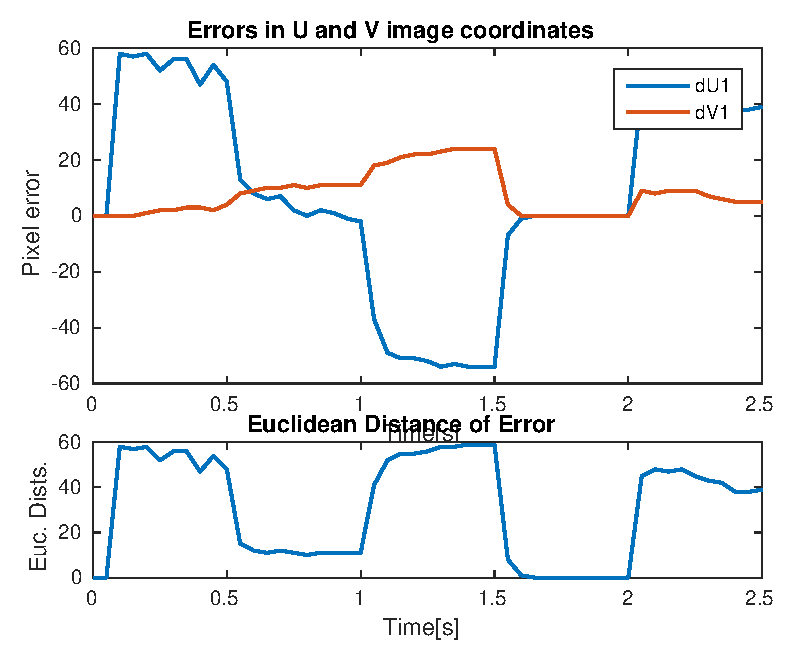
\includegraphics[width=0.49\linewidth]{fig/MediumSequence_dT50_1Pt_following_error_vs_time.eps}
	}\hfill
	\subfloat[Tracking 3 Points]
	{
		\label{fig:MediumSequence_dT50_MPt_following_error_vs_time}
		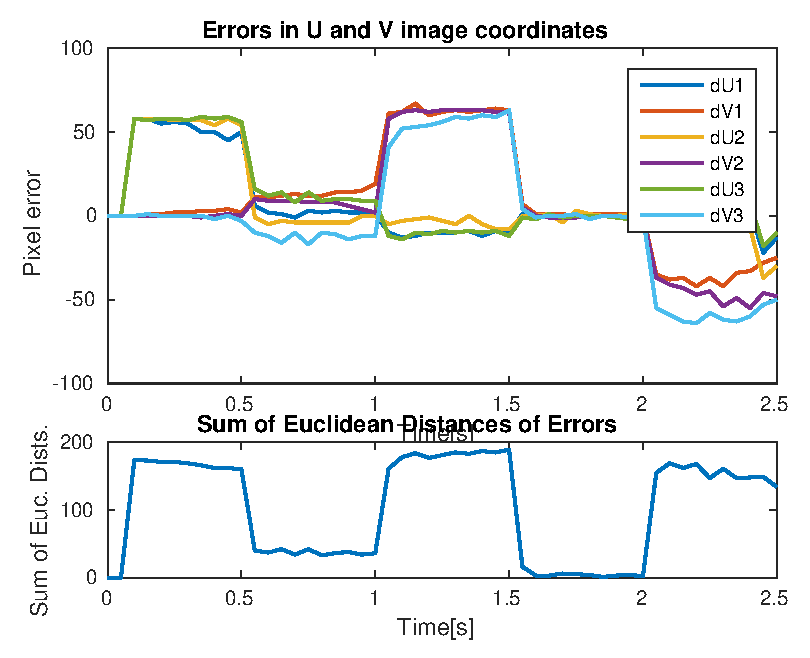
\includegraphics[width=0.49\linewidth]{fig/MediumSequence_dT50_MPt_following_error_vs_time.eps}
	}%
	\caption{Medium Sequence, \texttt{deltaT = 50} ms}
	\label{fig:MediumSequence_dT50_following_error_vs_time}
\end{figure}
\begin{figure}[!htp]
	% Maximum length
	\subfloat[Tracking Single Point]
	{
		\label{fig:MediumSequence_dT35_1Pt_following_error_vs_time}
		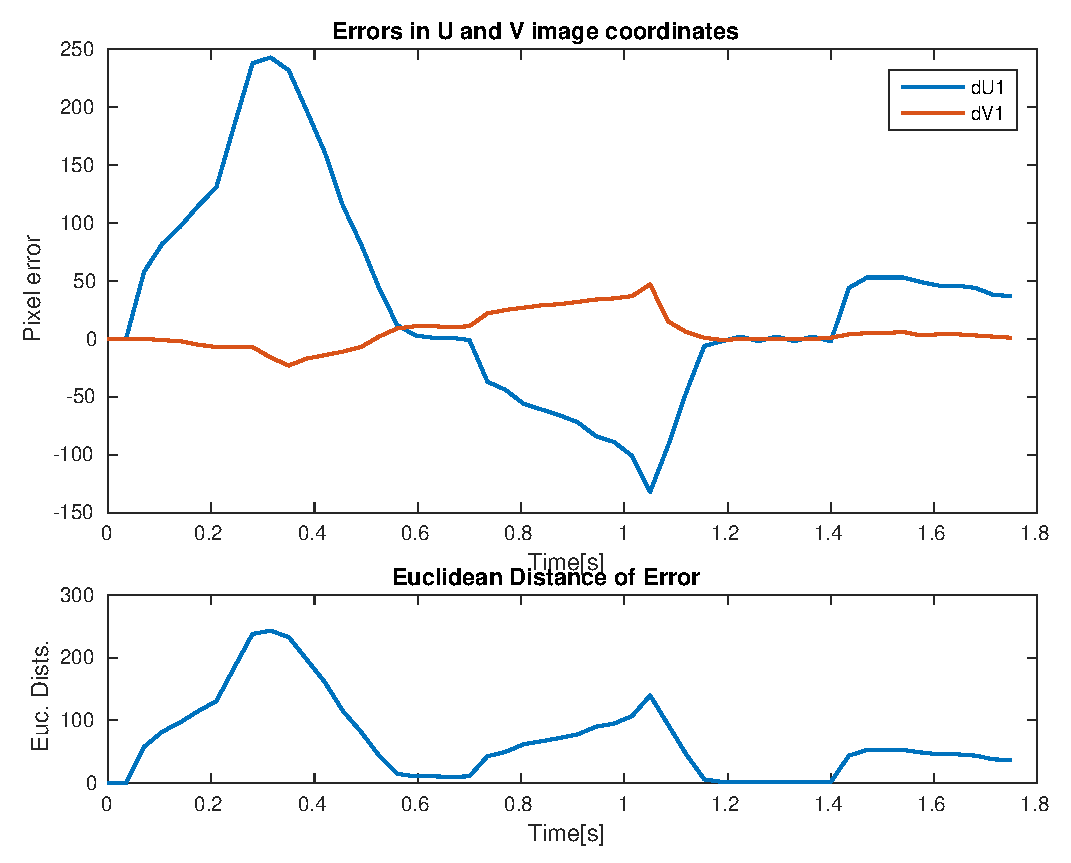
\includegraphics[width=0.49\linewidth]{fig/MediumSequence_dT35_1Pt_following_error_vs_time.eps}
	}\hfill
	\subfloat[Tracking 3 Points]
	{
		\label{fig:MediumSequence_dT35_MPt_following_error_vs_time}
		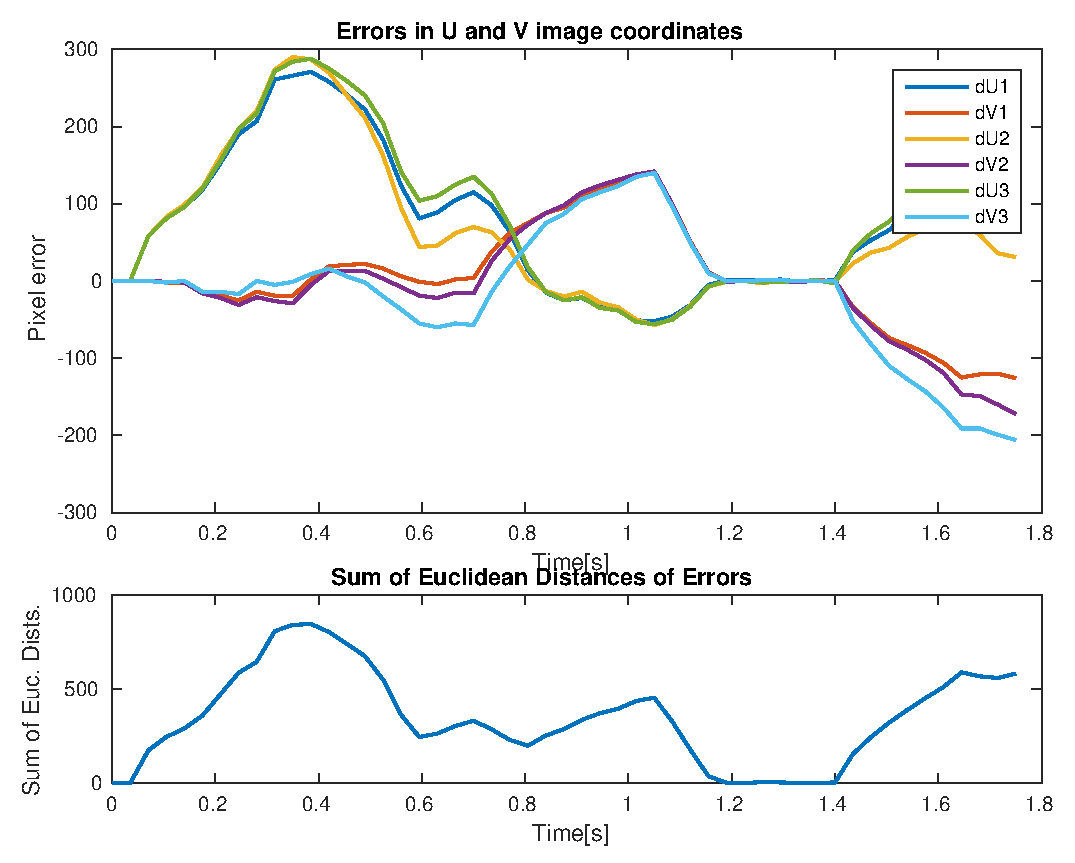
\includegraphics[width=0.49\linewidth]{fig/MediumSequence_dT35_MPt_following_error_vs_time.eps}
	}%
	\caption{Medium Sequence, \texttt{deltaT = 35} ms}
	\label{fig:MediumSequence_dT35_following_error_vs_time}
\end{figure}

%% Fast Sequence
Finally simulation for Fast sequence are plotted on the \ref{fig:FastSequence_dT100_following_error_vs_time} and \ref{fig:FastSequence_dT35_following_error_vs_time}.
\begin{figure}[!htp]
	% Maximum length
	\subfloat[Tracking Single Point]
	{
		\label{fig:FastSequence_dT100_1Pt_following_error_vs_time}
		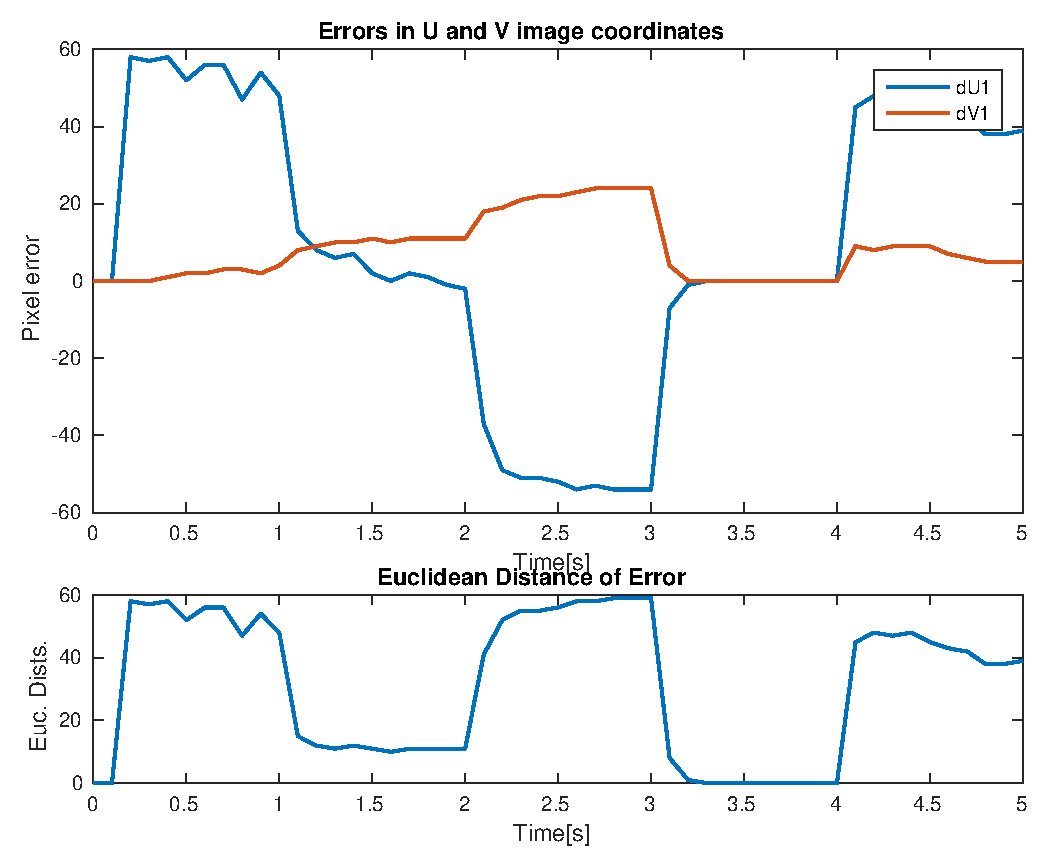
\includegraphics[width=0.49\linewidth]{fig/FastSequence_dT100_1Pt_following_error_vs_time.eps}
	}\hfill
	\subfloat[Tracking 3 Points]
	{
		\label{fig:FastSequence_dT100_MPt_following_error_vs_time}
		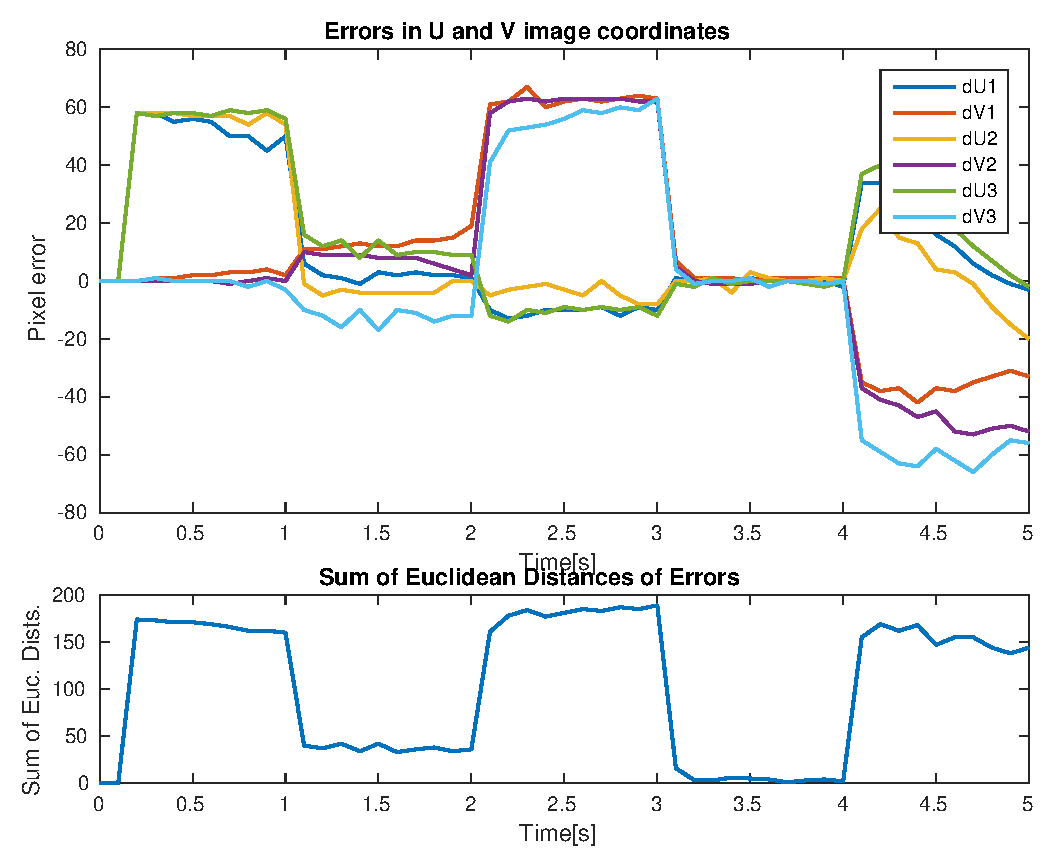
\includegraphics[width=0.49\linewidth]{fig/FastSequence_dT100_MPt_following_error_vs_time.eps}
	}%
	\caption{Fast Sequence, \texttt{deltaT = 100} ms}
	\label{fig:FastSequence_dT100_following_error_vs_time}
\end{figure}
\begin{figure}[!htp]
	% Maximum length
	\subfloat[Tracking Single Point]
	{
		\label{fig:FastSequence_dT35_1Pt_following_error_vs_time}
		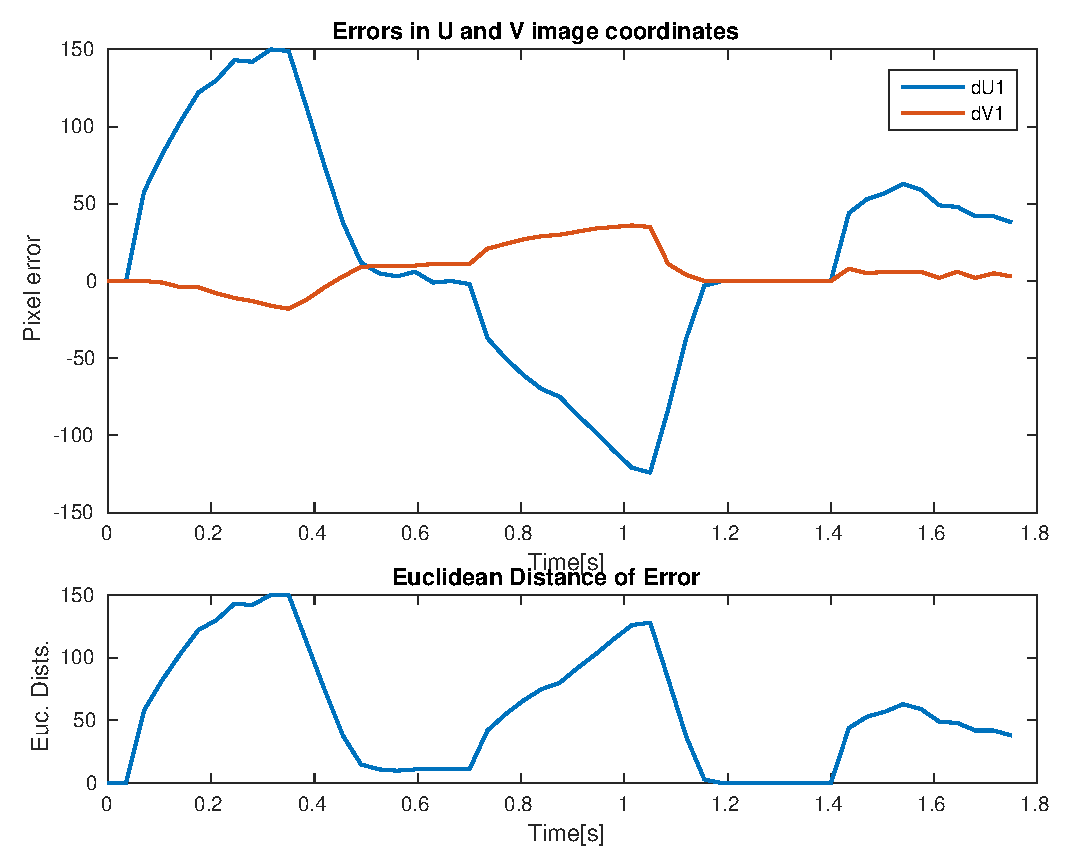
\includegraphics[width=0.49\linewidth]{fig/FastSequence_dT35_1Pt_following_error_vs_time.eps}
	}\hfill
	\subfloat[Tracking 3 Points]
	{
		\label{fig:FastSequence_dT35_MPt_following_error_vs_time}
		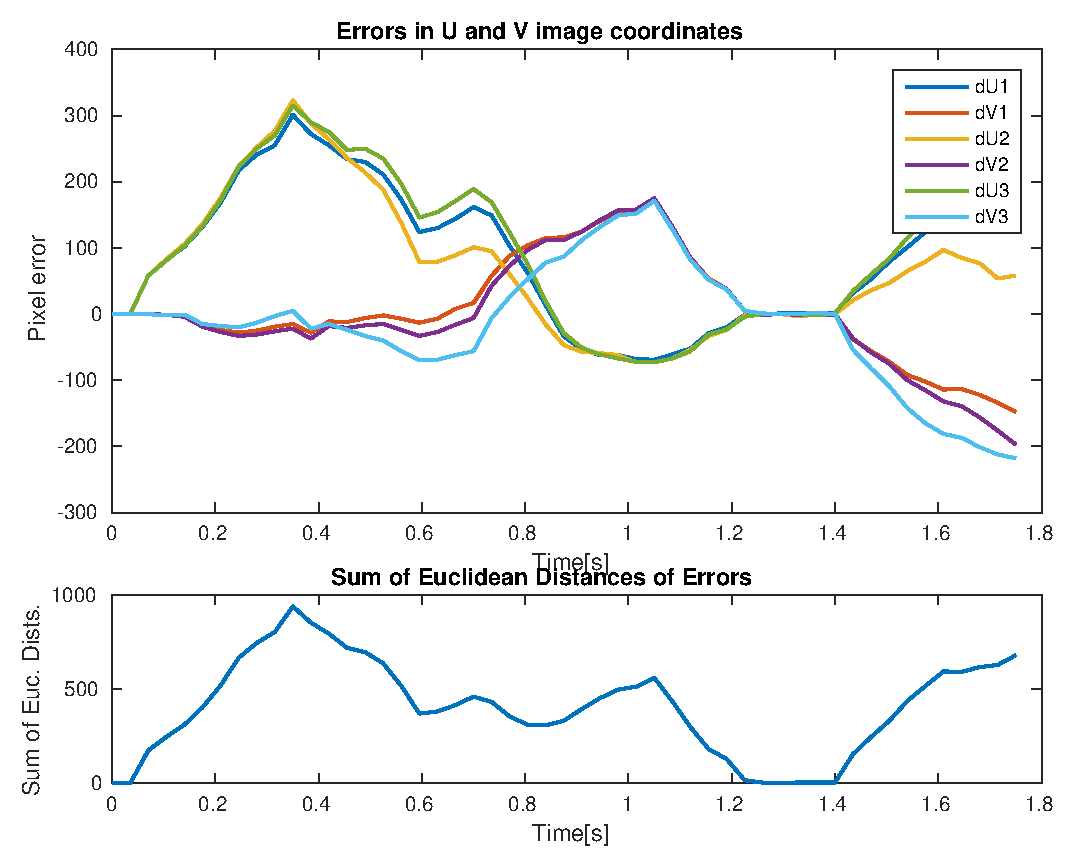
\includegraphics[width=0.49\linewidth]{fig/FastSequence_dT35_MPt_following_error_vs_time.eps}
	}%
	\caption{Fast Sequence, \texttt{deltaT = 35} ms}
	\label{fig:FastSequence_dT35_following_error_vs_time}
\end{figure}

\subsubsection*{Scaled joint positions and velocities}

\end{document}
